\documentclass[12pt,oneside]{book}
%------------------------------------------------
% Font/Symbol Options
%------------------------------------------------
\usepackage{mathptmx} % sets times fronts and mathsymbols
\usepackage{amssymb} % additional symbols not in mathptmx
\usepackage{mathtools} % package for improving math fonts
\usepackage[T1]{fontenc} % allows the use of glpys and special characters
\usepackage{relsize} % package for changing font size
\usepackage{xcolor} % foreground and background color management
\usepackage{soul} % package for hyphens, underlines, strike out, etc
\usepackage{enumerate} % allows numbered lists building on itemize
\usepackage{upquote} % sets quote style
\usepackage{moreverb} % allows the use of verbatim
\usepackage{gensymb} % provides gen symbols for math like \degree
\usepackage{ragged2e} % helps space words and hyphenate word wrap
\usepackage[titles]{tocloft} % control over the typography of the Table of Contents, List of Figures and List of Tables

% Colors used for cross references and table colors
\definecolor{linknavy}{rgb}{0,0,0.50196}
\definecolor{linkred}{rgb}{1,0,0}
\definecolor{linkblue}{rgb}{0,0,1}

%------------------------------------------------
% Float Options
%------------------------------------------------
\usepackage[pdftex]{graphicx} % improves includegraphics
\usepackage{caption} % customise the captions in floating environments like figure and table
\usepackage{subcaption}
\usepackage{xltabular} % keeps tabularx which helps with column management and but adds longtable
\newcolumntype{L}[1]{>{\raggedright\let\newline\\\arraybackslash\hspace{0pt}}m{#1}}
\newcolumntype{C}[1]{>{\centering\let\newline\\\arraybackslash\hspace{0pt}}m{#1}}
\newcolumntype{R}[1]{>{\raggedleft\let\newline\\\arraybackslash\hspace{0pt}}m{#1}}
\usepackage{booktabs} % high quality tables - allows toprule, midrule, etc
\usepackage{array} % extended implementation of the array and tabular environments which extends the options for column formats
\usepackage{float} % Improves the interface for defining floating objects such as figures and tables
\usepackage{placeins} % provides use of FloatBarrier for managing floats
% \usepackage{subfig} % provides ability to use subfigures
\usepackage{threeparttable} % allows for tablenotes
\usepackage{multirow} % allows split rows

% \usepackage{colortbl} % allows rows and cols of tables to be colored
% \definecolor{lbcolor}{rgb}{0.96,0.96,0.96}

%------------------------------------------------
% Crossref and Bibliography Options
%------------------------------------------------
\newcommand{\nopart}{\expandafter\def\csname Parent-1\endcsname{}} % To fix table of contents in pdf.

\usepackage{cite} %bibliography management
\usepackage{notoccite} % prevents references counting in figures/TOCs superceeding true numbering
\newcommand\notype[1]{\unskip} % allows skip of type for citing research reports
\usepackage[nottoc,notlof,notlot]{tocbibind} % Put the bibliography and index in the ToC
\usepackage[toc,page]{appendix} %defines appendix

%------------------------------------------------
% Output and Page Options
%------------------------------------------------

\renewcommand{\chaptername}{} % drops the word chapter
\renewcommand{\bibname}{References} % renames bibliography to references

\usepackage[pdftex,
        colorlinks=true,
        urlcolor=linkblue,     % \href{...}{...} external (URL)
        citecolor=linkred,     % citation number colors
        linkcolor=linknavy,    % \ref{...} and \pageref{...}
        pdfproducer={pdflatex},
        pdfpagemode=UseNone,
        bookmarksopen=true,
        plainpages=false,
        verbose]{hyperref} %handles cross references

\usepackage{geometry} % user interface to customize page layout

\setlength{\textwidth}{6.5in}
\setlength{\textheight}{9.0in}
\setlength{\topmargin}{0.in}
\setlength{\headheight}{0.pt}
\setlength{\headsep}{0.in}
\setlength{\parindent}{0.0in}
\setlength{\itemindent}{0.25in}
\setlength{\oddsidemargin}{0.0in}
\setlength{\evensidemargin}{0.0in}
% \setlength{\leftmargini}{\parindent} % Controls the indenting of the "bullets" in a list
\setlength{\cftsecnumwidth}{0.45in}
\setlength{\cftsubsecnumwidth}{0.5in}
\setlength{\cftfignumwidth}{0.45in}
\setlength{\cfttabnumwidth}{0.45in}
\setlength{\parskip}{1em}

\usepackage{fancyhdr}
\pagestyle{fancy}
\lhead{}
\rhead{}
\chead{}
\renewcommand{\headrulewidth}{0pt}

\usepackage{titlesec} % sets title stying
\titleformat{\chapter}[hang]{\normalfont\huge\bfseries}{\chaptertitlename\thechapter}{1em}{}
\titlespacing*{\chapter}{0pt}{-30pt}{20pt}

%------------------------------------------------
% Misc Optional Packages
%------------------------------------------------
\usepackage{setspace}
\usepackage{scrextend}
% \usepackage{calc} % simple arithmetic commands -- \setcounter,\setlength
% \usepackage{makeidx} % Create index at end of document
% \usepackage{lastpage} % Automatic last page number reference.
% \usepackage{xfrac} % Improves quality of fractions inline mathmode and in equations
% \usepackage{paralist} % inline lists
% \usepackage{varwidth} % variable width minipage
% \usepackage{listings} % allows user to typeset code inline
% \usepackage{tikz} % drawing package
\usepackage[version=4]{mhchem} % typesetting chemical molecular formulae and equations
% \usepackage{rotating} % rotated boxes (or floats, which are themselves boxes), and boxes always stay on one page.
% \usepackage{lscape} % continuous text (i.e., more than one page) set in landscape mode
% \usepackage{longtable} % allows tables to flow across pages

\usepackage{siunitx} %typsetting units
\sisetup{
    detect-all = true,
    input-decimal-markers = {.},
    input-ignore = {,},
    inter-unit-product = \ensuremath{{}\cdot{}},
    multi-part-units = repeat,
    number-unit-product = \text{~},
    per-mode = fraction,
    separate-uncertainty = true,
}

% \floatstyle{boxed}
% \newfloat{notebox}{H}{lon}
% \newfloat{warning}{H}{low}

% \newenvironment{conditions}
%   {\par\vspace{\abovedisplayskip}\noindent\begin{tabular}{>{$}l<{$} @{${}={}$} l}}
%   {\end{tabular}\par\vspace{\belowdisplayskip}}

%------------------------------------------------
% Title page definitions
%------------------------------------------------

\newcommand{\titlesigs}{\medskip
	\large \flushleft{UL Research Institutes} \\
	{Terrence R. Brady, President} \\
	{Christopher J. Cramer, Chief Research Officer} \\ \medskip
	\flushleft{Fire Safety Research Institute \\
		{Steve Kerber, Vice President and Executive Director} \\
		\hspace{1in} \\}}


\newcommand{\titleA}{\flushleft{\huge\bf{\vartitle}}}
\newcommand{\titleB}{\vspace{.5in}\flushleft{\large\flushleft{\varauthors\vspace{0.2in}\varaddress\vspace{0.2in}\vardate}}}
\newcommand{\titleC}{\vspace{.3in}\flushleft{\large\flushleft{This publication is available free of charge from:\\ \vardoi}}}
\newcommand{\titleD}{
	\begin{minipage}{0.35\textwidth}
		\begin{flushleft}
			
\includegraphics[width=1\textwidth]{../Bibliography/UL_RI}
		\end{flushleft}
	\end{minipage}
	\hfill
	\begin{minipage}{0.5\textwidth}
		\begin{flushright}
			
\includegraphics[width=1.25in]{../Bibliography/FSRI_Logo_white}
		\end{flushright}
	\end{minipage}
}
\newcommand{\titleE}{\scriptsize\flushleft{\textcopyright \the\year{}. UL Research Institutes. All rights reserved.}}


\newcommand{\forceindent}{\leavevmode{\parindent=1em\indent}}
% -----------------------------------------------
% Set Report Title and Authors
% -----------------------------------------------
\newcommand{\vartitle}{Materials and Products Database - Technical Reference Guide\\}
\newcommand{\vardate}{\today \\}
\newcommand{\varauthors}{Mark McKinnon \\
						Craig Weinschenk \\
						Daniel Madrzykowski \\}
\newcommand{\varaddress}{Fire Safety Research Institute \\
	UL Research Institutes\\
	Columbia, MD 21045 \\}
\newcommand{\vardoi}{\url{https://dx.doi.org/10.54206/XXXXXXXX}}


\begin{document}
\pagenumbering{gobble}
\bibliographystyle{unsrturl}
\urlstyle{rm}
\hypersetup{pageanchor=false}

% Custom Commands
\newcommand*\degC[1]{{#1}~\textdegree C}  % \degC{22}

%------------------------------------------------
% Title Page 1
%------------------------------------------------
\begin{minipage}[t][9in][s]{6.25in}
\titleA
\titleB
\titleC
\vfill
\titleD
\titleE
\end{minipage}

%------------------------------------------------
% Blank page between Title Pages
%------------------------------------------------

\newpage
\hspace{5in}
\newpage

%------------------------------------------------
% Title Page 3
%------------------------------------------------

\begin{minipage}[t][9in][s]{6.25in}
\pagenumbering{gobble}
\titleA
\titleB
\titleC
\vfill
\titlesigs
\titleD
\titleE
\end{minipage}
\newpage

\begin{minipage}[t][9in][s]{6.25in}

\flushleft{In no event shall UL Research Institutes be responsible to anyone for whatever use or non-use is made of the information contained in this Report and in no event shall UL Research Institutes, its employees, or its agents incur any obligation or liability for damages including, but not limited to, consequential damage arising out of or in connection  with the use or inability to use the information contained in this Report. Information conveyed by this Report applies only to the specimens actually involved in these tests. UL Research Institutes has not established a factory Follow-Up Service Program to determine the conformance of subsequently produced material, nor has any provision been made to apply any registered mark of UL to such material. The issuance of this Report in no way implies Listing, Classification or Recognition by UL Enterprises and does not authorize the use of UL Listing, Classification or Recognition Marks or other reference to UL Enterprises on or in connection with the product or system.
}

\vspace{3in}
\vfill
\hspace{1in}

\end{minipage}

\newpage
\hypersetup{pageanchor=true}

\newpage
\frontmatter

\pagestyle{plain}
\pagenumbering{roman}

\cleardoublepage
\phantomsection
\tableofcontents

\cleardoublepage
\phantomsection
\addcontentsline{toc}{chapter}{List of Figures}
\listoffigures

\cleardoublepage
\phantomsection
\addcontentsline{toc}{chapter}{List of Tables}
\listoftables

\chapter*{\centering Acknowledgments}

\begin{table}[!ht]
	\centering
	\caption*{Project Technical Panel}
	\begin{tabular}{ll}
		\toprule[1.5pt]
		Name & Affiliation \\ 
		\midrule
		Vyto Babrauskas	 	& Fire Science and Technology Inc \\
		Ernest Barile	 	& Philadelphia Fire Department \\
		Nicole Brewer	 	& Portland Fire \& Rescue \\
		Morgan Bruns	 	& St. Mary's University of Texas \\		
		Steve Carman 		& Carman \& Associates Fire Investigation, Inc \\
		Paul Claflin 		& Bureau of ATF, Fire Investigation \& Arson Enforcement Division \\
		Jason Dress	    	& Bureau of ATF, Fire Research Laboratory \\
		Adam Friedman	    & Bureau of ATF, Fire Research Laboratory\\
		Brian Geraci 		& Maryland State Fire Marshal \\
		Barry Grimm 		& International Association of Arson Investigators \\
		Brian Lattimer	 	& Virginia Polytechnic Institute and State University \\
		Chris Lautenberger	& Reax Engineering \\
		Kevin McGrattan 	& National Institute of Standards and Technology \\ 
		Tom Sabella 		& Fire Department City of New York, Retired \\
		Stanislav Stoliarov	& University of Maryland \\ 
		\bottomrule[1.25pt]
	\end{tabular}
\end{table}

\chapter*{List of Abbreviations}

\begin{tabbing}
\hspace{1.5in} \= \\
DSC 	\> Differential scanning calorimetry \\
FDS	    \> Fire Dynamics Simulator \\
FSRI    \> Fire Safety Research Institute \\
FTIR 	\> Fourier transform infrared spectrometer \\
HFM 	\> Heat flow meter \\
IS 		\> Integrating sphere \\
MCC 	\> Microscale combustion calorimetry \\
NIJ 	\> National Institute of Justice \\
NIST    \> National Institute of Standards and Technology \\
NLLS    \> Nonlinear least squares \\
SRM 	\> Standard reference material \\
STA 	\> Simultaneous thermal analyzer \\
TGA 	\> Thermogravimetric analysis \\
\end{tabbing}

\newpage

\pagenumbering{arabic}
\setcounter{page}{1}

\newpage
\mainmatter
\newpage

\chapter{Introduction}
\label{sec:introduction}

For the past several years, the NIJ Technology Working Group's Operational Requirements (TWG ORs) for Fire and Arson Investigation have included several scientific research needs that require improved knowledge of properties of materials that are common in the built environment, and therefore likely to be involved in a fire scene. The specific areas of research include: adequate materials data inputs for accurate computer models, understanding the effect of materials properties on the development and interpretation of fire patterns, and evaluation of incident heat flux profiles to walls and neighboring items in support of fire model validation. Each of the three aforementioned research topics rely, in part, on accurate knowledge of the physical conditions of a material prior to the fire, how the material will respond to the exposure of heat, and how it will perform once it has ignited. The project described herein has made advancements in terms of collecting experimental data and property information on a multitude of materials commonly encountered in the built environment for the purpose of making the data publicly available and easily accessible to fire investigators, fire protection engineers, and fire researchers.

The information presented in this technical reference guide includes a description of the experimental procedures, and data analysis approaches including estimated uncertainty in the measurements that have been adopted to collect the data for selected materials. The analytical procedures through which the properties were extracted from the collected data are presented to provide users of the database with context for the available data. There is no expectation or requirement that users of the database utilize the same analytical methods that are described in this work, and, as such, they constitute technically defensible recommendations for the fire modeling and investigation communities.

\chapter{Experimental Procedures}
\label{sec:experimental}

The set of experiments used to measure the data from which properties were determined may be divided according to the size of the specimen on which the measurement is made. The experimental procedures presented in this section are divided into general properties, which are unaffected by the scale of the specimen, milligram-scale experiments, which are designed to observe thermal degradation processes isolated from transport processes, and bench-scale experiments, which are designed to incorporate all the most important physics of pyrolysis at the smallest scale at which the boundary conditions may be controlled.

\section{General Properties}
\label{sec:general_properties}

In the context of this work, general properties refers to the properties that are typically unaffected by the scale of the experimental sample. These properties include the density and moisture content of the sample.

\subsection{Density}
\label{sec:density}

The density of all materials was determined by directly measuring the mass and volume of at least three samples. Prior to measurement, samples were prepared into prismatic geometries to make volume measure straightforward. After preparing prismatic samples, the samples were conditioned according to the specific protocol for each experimental method and the volume and mass of the samples were measured.  

\subsection{Moisture Content}
\label{sec:moisture_content}

The temperature and humidity at which materials are stored and have reached equilibrium prior to ignition or being tested to measure a specific property have a marked effect on the thermo-physical properties and the fire response of the material. When possible, the moisture content of the sample material was measured prior to standard testing. For tests conducted with the heat flow meter (HFM), which is a non-destructive test, the density of the samples was measured, the tests were conducted, and then samples were stored in an oven at a temperature of \degC{105} for a minimum of 48 hours until the mass of the sample stabilized. The resulting samples were considered to have reached equilibrium with the dry environment in the oven and the density of the samples was measured. The difference in mass of the samples in the dried and non-dried state was attributed to absorbed water and was directly used to calculate the moisture content of the non-dried samples.

Material samples were conditioned for cone calorimeter tests in a conditioning chamber held at 50\% relative humidity (RH) and \degC{23} for a minimum of 48 hours and long enough for the mass of the samples to stabilize. The moisture content of the cone calorimeter sample was determined relative to the measured density of the dried heat flow meter samples.

The moisture content of material samples tested with the simultaneous thermal analyzer (STA) was determined directly from the measured mass. The mass of the sample is measured with respect to temperature in STA tests, so the mass of the sample lost from the beginning of the test to approximately \degC{100} was attributed to moisture loss and was directly used to determine the moisture content of the material. 

\section{Milligram-scale Experiments}
\label{sec:mg_scale_exp}

Milligram-scale experiments are also known as thermal analysis experiments and rely on the assumption that the sample is sufficiently small that thermal and mass gradients are negligible throughout the experiment, which is equivalent to the assumption that transport processes are also negligible. Thermal analysis experiments typically consist of a sample with a mass on the order of a few milligrams heated along a well-defined temperature program in a well-defined gas atmosphere. One or more quantities are measured during the experiment, and when more than one quantity is measured simultaneously, the term simultaneous thermal analysis is applied. Thermogravimetric analysis (TGA) involves the measurement of mass during a thermal analysis experiment, differential scanning calorimetry (DSC) is the measurement of heat flow rate during a thermal analysis experiment, and micro-scale combustion calorimetry (MCC) is an experimental technique in which a sample is gasified in the thermal analysis experiment and the heat evolved from combustion of the produced gases and vapors is measured. The database includes data collected in STA experiments in which TGA and DSC were conducted simultaneously as well as data from MCC experiments. 

\subsection{Simultaneous Thermal Analysis}
\label{sec:sta}

A NETZSCH STA 449 Jupiter F3 Simultaneous Thermal Analyzer (STA), pictured in Figure~\ref{fig:STA_apparatus}, was used to simultaneously conduct TGA to determine the kinetics of thermal degradation as well as DSC to determine specific heat capacities, the heat of reaction, and the heat of gasification for materials. The STA incorporated a heat flux style DSC measurement. The apparatus consists of a twin-style sample carrier with a space for a reference crucible and a sample crucible. The crucibles are ideally weight-matched and consistently placed in the same position on the carrier to ensure consistent heat flow rate measurements. A thermocouple welded to the bottom of each carrier position measures the temperature of each crucible. The carrier system is encompassed in a furnace and the apparatus incorporates mass flow controllers to maintain well-characterized gaseous composition and flow conditions while the furnace maintains a well-characterized temperature.  

\begin{figure}[!ht]
\centering
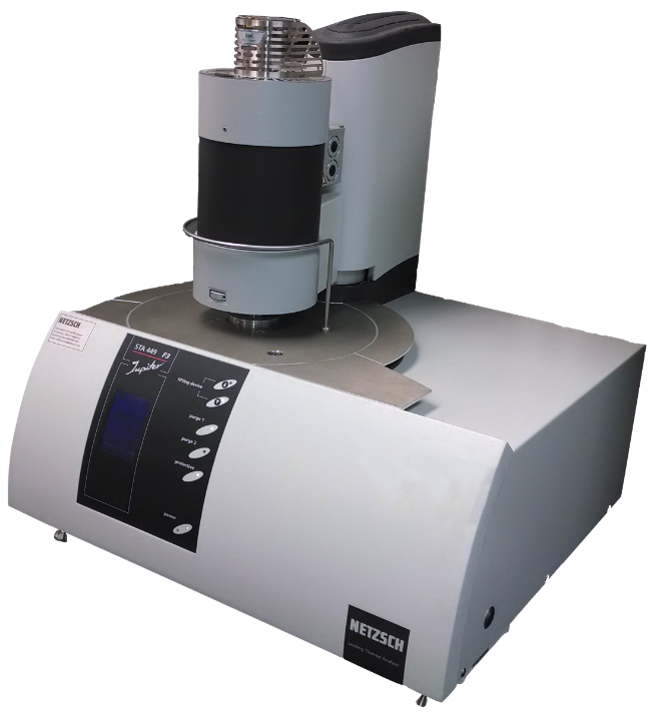
\includegraphics[width=.75\columnwidth]{Figures/STA.png}
\caption[Image of the Simultaneous Thermal Analyzer (STA) Apparatus]{Image of the simultaneous thermal analyzer (STA) apparatus.}
\label{fig:STA_apparatus}
\end{figure}

\subsubsection{Sample Preparation}

The material samples were prepared into powders using a cryogenic mixing ball mill (shown in Figure~\ref{fig:cryomill}) which ground the samples for a minimum of ten minutes. This ensured that samples were homogeneous and representative of the bulk material and guaranteed sufficient thermal contact between the sample and the crucible. Good thermal contact is necessary for accurate heat flow measurement because the principle of a heat flux DSC uses thermocouple measurements from the center of the bottom surface of the crucible to determine the heat flow rate.

\begin{figure}[!ht]
\centering
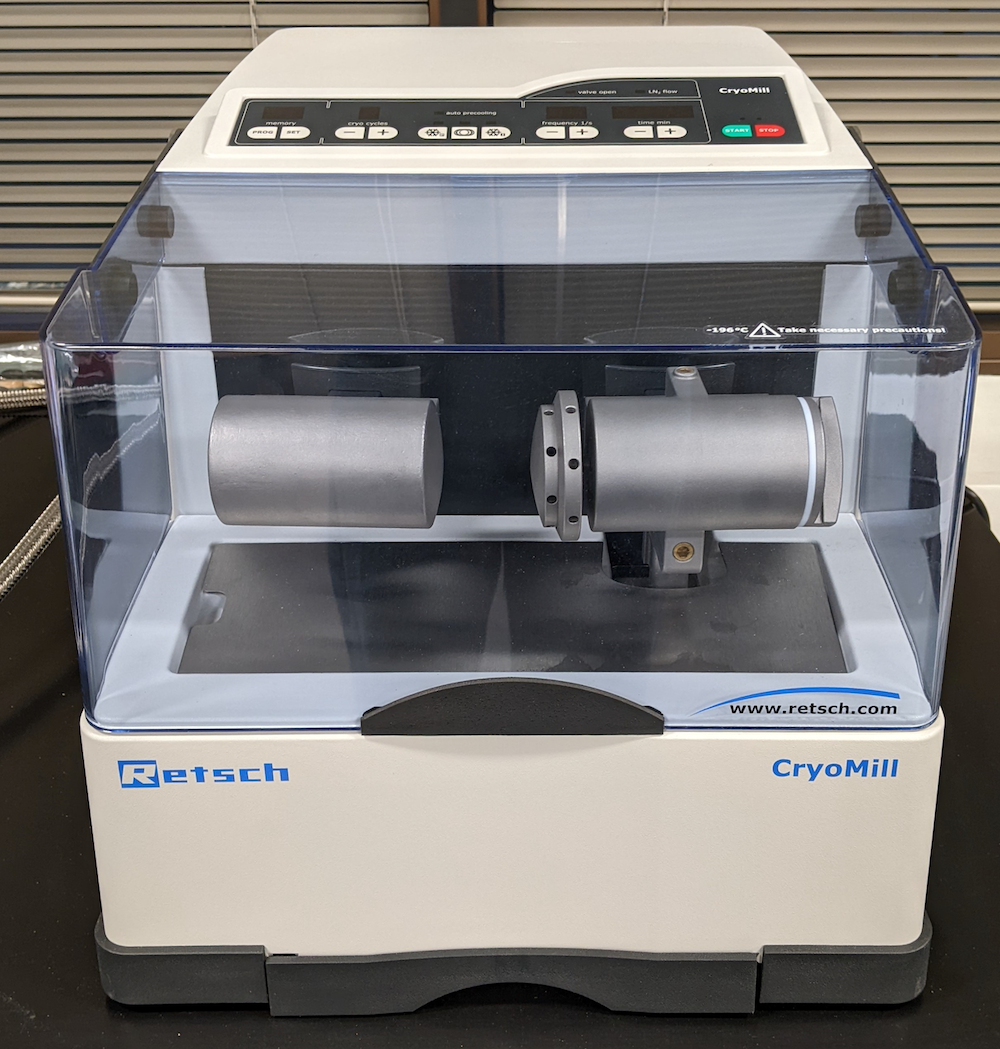
\includegraphics[width=.75\columnwidth]{Figures/Cryomill.png}
\caption[Image of the Cryogenic Mixing Ball Mill Used for Thermal Analysis Sample Preparation]{Image of the cryogenic mixing ball mill used for thermal analysis sample preparation.}
\label{fig:cryomill}
\end{figure}

Powdered samples were stored in a desiccator in the presence of Drierite for a minimum of 48 hours prior to STA experiments to minimize the impact of moisture of the experiments. Although the desiccator maintained an environment below 10\% RH, samples generally still had some non-zero moisture content which was determined as outlined in Section~\ref{sec:moisture_content}. An photograph of a representative powdered sample and a platinum crucible are provided in Figure~\ref{fig:sta_sample} to show the relative scale of the sample.

\begin{figure}[!ht]
\centering
\includegraphics[width=.75\columnwidth]{Figures/STA_Sample_Prep.png}
\caption[Image of the Powdered Sample Prepared through Cryogenic Grinding for STA Experiment]{Image of the powdered sample prepared through cryogenic grinding for STA experiment.}
\label{fig:sta_sample}
\end{figure}

\subsubsection{Calibration}

The data presented in the database were collected from STA tests conducted with two different types of furnaces. At the beginning of the project, the only furnace available was a silicon carbide (SiC) furnace, and later in the project a platinum (Pt) furnace became available. The Pt furnace provided greater repeatability in the temperature profile and higher sensitivity heat flow rate measurements than the SiC furnace. 

The measured temperature of the furnace and the voltage difference measured between the sample and reference crucible thermocouples was correlated to heat flow rates through a calibration procedure that involved the known onset temperature for melting and heats of fusion for a set of pure organic compounds and anhydrous salts. A five-point temperature calibration was conducted in general accordance with the procedure described in ASTM E967~\cite{ASTM_E967}. A five-point sensitivity curve was constructed from an exponentially decaying third-degree polynomial using data collected generally according to the procedure described in ASTM E968~\cite{ASTM_E968}. 

The calibration procedure was performed at least every 200 temperature cycles in the STA. The temperature calibration took a linear form for the SiC furnace and the standard deviation of the residuals of that linear regression was at most \degC{0.9} for the calibrations applied to the data presented in the database. The temperature correction for the Pt furnace took on a second-degree polynomial form with the standard deviation of residuals less than \degC{0.1}. The sensitivity calibration curve had a standard deviation of the residuals of $\pm$ 0.05 \si{\micro V/mW} for the SiC furnace and $\pm$ 0.02 \si{\micro V/mW} for the Pt furnace. These standard deviations corresponded to approximately $\pm$7\% in the heat flow curve over the temperatures of interest in the SiC furnace and approximately $\pm$2\% in the heat flow rate curve over the temperatures of interest in the Pt furnace. The STA mass balance system was serviced annually and this service consisted of a recalibration of the balance. 

\subsubsection{Experimental Procedure}

Tests were conducted at heating rates of 3, 10, and 30 \degC{}/min with an initial temperature of \degC{50} and a maximum temperature chosen to ensure decomposition was completed (typically approximately \degC{650}. The crucible lid was placed on the sample crucible and the edge of the sample crucible was marked to ensure consistent orientation of the crucible relative to the sample carrier. All the data currently in the database were collected in experiments conducted in a nitrogen atmosphere with a total flow rate of 70~mL/min. The temperature program for the STA experiments consisted of an isotherm for 10 minutes at \degC{50} followed by a linear increase in temperature at the constant set point heating rate to the maximum temperature set point followed by a 5 minute isotherm at the final temperature. The experiment was conducted without a sample in the crucible to collect correction data. The entire experiment was repeated with a sample in the crucible to collect data on the sample material. The sample preparation procedure for STA tests involved spreading a powdered sample of the material to be tested with a mass of 4.0$\pm$0.1 mg evenly across the bottom of a platinum-rhodium crucible. Analysis involved subtracting the correction data from the sample data. 

\subsubsection{Experimental Uncertainty}

The raw quantities measured with the STA are the mass of the sample system and the voltage difference between the thermocouple signals collected at the sample and reference crucibles. Because the mass of the carrier, crucibles, and sample measured in the experiment were corrected with a test conducted immediately before the sample test, it is expected that the uncertainty in the measured mass was minimal. This uncertainty was evaluated by comparing the masses measured in consecutive tests (sample and correction tests) in temperature ranges at which no physical mass loss occurred (measured mass variations were caused by drift or geometric differences). The maximum difference between the measured mass curves in consecutive tests for general polymers was determined as 0.08 mg, which constitutes an uncertainty in the mass signal of $\pm$2\% for the experimental data presented in the database. The uncertainty in the mass measurement may be compared to the variability in the residual mass of the char yielded in STA experiments at \degC{650} which was approximately $\pm$5\%.

\subsection{Micro-scale Combustion Calorimetry}
\label{sec:sta}

A Fire Testing Technology microscale-combustion calorimeter (MCC), shown in Figure~\ref{fig:MCC_apparatus}, was used to measure the heat release rate of the pyrolyzate evolved during pyrolysis of the sample material. The apparatus consists of a flat sample platform sized for a single crucible. Experiments were performed in general accordance with ASTM D7309~\cite{ASTM_D7309}. During a test, the crucible is moved into a furnace region that is constantly purged with nitrogen gas. A thermocouple bead on the sample platform ensures the temperature of the sample follows the set point temperature. The evolved pyrolyzate is allowed to flow to a combustion chamber which is held at \degC{900} and where excess oxygen is injected to ensure the pyrolyzate undergoes complete combustion. The gas effluent flows to an oxygen sensor where the decrease in oxygen concentration is measured and related to the heat release rate through the principle of oxygen-consumption calorimetry. 

\begin{figure}[!ht]
\centering
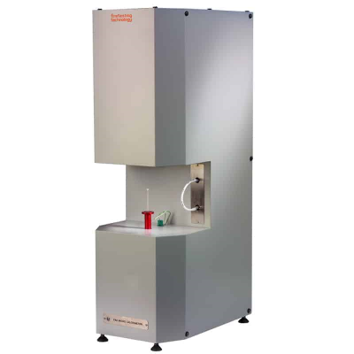
\includegraphics[width=.75\columnwidth]{Figures/MCC.png}
\caption[Image of the Micro-Scale Combustion Calorimeter (MCC) Apparatus]{Image of the micro-scale combustion calorimeter (MCC) apparatus.}
\label{fig:MCC_apparatus}
\end{figure}

\subsubsection{Sample Preparation}

The material samples were prepared into powders using a cryogenic mixing ball mill which ground the samples for a minimum of ten minutes. This ensured that samples were homogeneous and representative of the bulk material and guaranteed sufficient thermal contact between the sample and the crucible. This sample preparation method was identical to the samples prepared for the STA experiments to ensure a comparison between the data collected in each experiment could be directly compared.

Powdered samples were stored in a desiccator in the presence of Drierite for a minimum of 48 hours prior to MCC experiments to minimize the impact of moisture of the experiments.

\subsubsection{Calibration}

The sample temperature measured by the MCC system was calibrated by comparing the onset temperature of melting measured with the sample thermocouple to literature values for a set of pure metals. The temperature correction applied to the measured temperature was defined by a second-degree polynomial. The coefficients were unique to the heating rate and the crucible material and were measured with a heating rate of 30~\degC{}/min and the ceramic crucibles provided by the manufacturer. The heat release rate time delay was calibrated by pulsing oxygen into the system and monitoring the time between the onset of oxygen flow and the oxygen sensor registering an increase in oxygen concentration. The oxygen sensor was calibrated daily during testing by introducing a known flow rate of oxygen into the system and measuring the oxygen concentration with the oxygen sensor. The voltage from the oxygen sensor at no oxygen flow was recorded as the zero point and the voltage at the high limit was recorded when 25~mL/min of oxygen at standard temperature and pressure (STP) was flowed into the system. After the oxygen sensor was calibrated and at least once daily, powdered polystyrene was tested according to the full MCC test procedure and the heat of combustion, the peak HRR, and the temperature corresponding to the peak HRR were compared against literature values to ensure the MCC system was accurately measuring HRR.

\subsubsection{Experimental Procedure}

A powdered sample of the material to be tested with a mass of 4.0$\pm$0.1 mg was spread evenly across the bottom of the ceramic crucible. The sample and crucible mass were measured prior to testing. Tests were conducted with a heating rate of 30 \degC{}/min with an initial temperature of \degC{50} and a maximum temperature that was typically approximately \degC{750}). Tests were conducted with samples in ceramic crucibles with no lids to ensure there was no added resistance to flow of pyrolyzate gases and vapors from the sample to the combustion chamber. All the data currently in the database were collected in experiments conducted in a nitrogen atmosphere with a total flow rate of 80~mL/min. The temperature of the combustion chamber was set to \degC{900} and the oxygen flow rate to the combustion chamber was 20~mL/min. After the sample reached the maximum temperature, the sample and crucible were allowed to cool and the mass of the crucible and residue was measured to determine the char yield. 

\subsubsection{Experimental Uncertainty}

The MCC uses measurements of temperature, oxygen concentration, and an independent measurement of mass for determination of the HRR with respect to temperature and the effective heat of complete combustion. The typical maximum expanded uncertainty in thermocouple measurements of temperature is $\pm$\degC{2} at \degC{900}. For the majority of the temperature program experienced by the sample specimen, this equates to an uncertainty of less than $\pm$1\%. The estimated uncertainty in mass measurements made with the analytical balance was $\pm$0.01~mg. Because the MCC method requires the difference between the initial mass and the residual mass, and this difference has a maximum of 4~mg and a minimum of approximately 3~mg for the materials that are currently in the database, the relative uncertainty can be assumed to be approximately $\pm$1\%.

The uncertainty in the determination of HRR using flow calorimetry with the MCC depends on the oxygen concentration measurement, the density of oxygen entering the oxygen sensor, and the flow rate of the gases that flow to the oxygen sensor, and the heat of combustion of oxygen with hydrocarbon fuels. The accuracy of the oxygen concentration measurement using an electrochemical sensor was reported as $\pm$1\%. It is assumed that the oxygen concentration is measured on gases at room temperature because the gases flow from the combustion chamber, through driers and filters prior to reaching the oxygen sensor. The density of the oxygen at the sensor is assumed to be the value at \degC{25} and the density scales with the ratio of the actual absolute temperature to the absolute temperature of the ideal state. Assuming the uncertainty in the temperature is only due to the uncertainty in the thermocouple measurement, the density of oxygen has an uncertainty of $\pm$1\%. The ASTM standard specifies that the accuracy of the flow meter be $\pm$1\% at full scale. The coefficient of variation of the heat of combustion of oxygen with hydrocarbon fuels is $\pm$5\%. Combining theses systematic uncertainties yields an expanded systematic uncertainty of approximately $\pm$6.5\% in the HRR measurement.

An inter-laboratory study which measured the HRR of five materials using the MCC was conducted to investigated repeatability and reproducibility of the measurements made when conducting tests with the apparatus following the standard method outlined in ASTM D7309. According to ASTM E691,\emph{Practice for Conducting an Interlaboratory Study to Determine the Precision of a Test Method}, the repeatability is defined as the expected range about the measured value that encompasses 95\% of the data when the test is repeated immediately after the measurement is made. The reproducibility is defined as the same metric when a different laboratory repeats the measurement. The study showed a repeatability standard deviation of approximately $\pm$0.3~kJ/g and a reproducibility standard deviation of approximately $\pm$1.5~kJ/g for the total heat release. For a material with a total heat release of 25~kJ/g, this equates to an expanded repeatability (k=2) of $\pm$2.4\% and an expanded reproducibility of $\pm$12\%. Additional results are presented in the literature~\cite{ASTM_D7309,MCC_ILS}. 

\section{Bench-scale Experiments}
\label{sec:bench_scale_exp}

Bench-scale experiments were conducted to characterize thermal transport properties, optical properties, and to collect validation data on the materials in the database. Experiments were conducted according to ASTM C518~\cite{ASTM_C518} to measure the thermal conductivity and according to a modified version of ASTM C1784~\cite{ASTM_C1784} to determine the specific heat capacity of the material. An integrating sphere (IS) accessory was used with the FTIR spectrometer to determine the spectral reflectivity from which the spectral emissivity was calculated for all the materials in the database generally according to ASTM E903~\cite{ASTM_E903}. The IS was also used to measure spectral transmission from which absorption coefficient was calculated. Transmission was only measured for a subset of materials that were suspected of allowing transmission and in-depth absorption of infrared radiation. Experiments were conducted with the cone calorimeter in general accordance with ASTM E1354~\cite{ASTM_E1354} to measure the heat release rate per unit area (HRRPUA), time to ignition, and smoke yield of the material given a set point incident heat flux. Cone calorimeter data may also serve as validation data for the complete set of properties measured through all other experimental procedures.

\subsection{Heat Flow Meter}
\label{sec:hfm}

A TA instruments FOX 200 HFM, shown in Figure~\ref{fig:HFM_apparatus} was used to measure the thermal conductivity and specific heat capacity of the materials in the database. The apparatus consists of two plates between which a 200~mm x 200~mm sample specimen is placed during a test. During a test, an actuator above the upper plate moves the upper plate until contact is made between the upper plate and the sample specimen. The instrument measures the distance between the two plates as the thickness of the material. The temperature of each plate is controlled with Peltier coolers and resistance heaters. The heat flow through each plate is measured with thermopiles and the measured quantity may be related to the thermal conductivity or the specific heat capacity of the material, depending on the relationship between the set temperatures of each plate.

\begin{figure}[!ht]
\centering
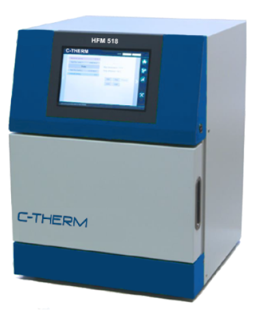
\includegraphics[width=.75\columnwidth]{Figures/HFM.png}
\caption[Image of the Heat Flow Meter (HFM) Apparatus]{Image of the heat flow meter (HFM) apparatus.}
\label{fig:HFM_apparatus}
\end{figure}

\subsubsection{Sample Preparation}

Samples were cut square with a side of 0.20 m and tested immediately in the unconditioned as-received state. After testing in the as-received state, the sample specimens were dried in a convection oven at a temperature of \degC{105} for a minimum of 48 hours until the mass of the dried samples no longer changed. If the mass of the dried samples did not change from the as-received state, it was assumed the as-received state did not hold any absorbed moisture. The mass of each sample and the calculated density was recorded prior to each HFM test.

Sample materials that could not be made into specimens with the desired outside dimensions were cut as large as possible and the remainder of space in the HFM was filled with the same material. This was possible because the sensing surface was confined to the central 0.075~m x 0.075~m, and the role of the filler material was to minimize unnatural thermal gradients at the edges of the samples. Using the same material as the test specimen minimized the affect of thermal transport across the interface between the sample specimen and the fillers.

\subsubsection{Calibration}

The HFM was calibrated with several calibration standards procured from or that could be traced back to the National Institute of Standards and Technology (NIST). A NIST 1453 expanded polystyrene standard reference material (SRM) was initially used to calibrate the HFM for thermal conductivity determination. The effective temperature range of the 1453 SRM was approximately \degC{8} to \degC{45}, which defined the upper and lower limits of thermal conductivity determination when using the 1453 SRM. To increase this temperature range, a NIST 1450e fibrous glass board SRM was procured to calibrate the HFM for thermal conductivity determination. The effective temperature range of the 1450e SRM was approximately 7 to \degC{87}. The maximum plate temperature that could be achieved with the HFM used for measure data presented in the database was \degC{75}. Because the effective temperature of the material at which the thermal conductivity is assigned is the mean between the plate temperatures, this limited the maximum mean temperature of the sample for thermal conductivity measurement to \degC{65} with the 1450e SRM.

A NIST 1450b SRM (fibrous glass board) calibration that was loaded on the apparatus when it was received from the manufacturer was used for specific heat capacity determination. The effective temperature range of the 1450b SRM was -13 to \degC{57}. The specific heat capacity determination also required a correction for the heat capacity of the plates. This was determined by conducting tests with no sample between the plates. A proprietary program developed by TA Instruments was used to subtract the heat capacity of the plates and to calculate the specific heat capacity of the sample specimen. 

\subsubsection{Experimental Procedure}

The ASTM C518 tests consisted of setting the temperatures of the cold and hot plates such that there was a difference of \degC{20} and allowing the system to achieve equilibrium. When using the 1453 SRM, the first set of temperatures were \degC{5} and \degC{25} and the second set were \degC{35} and \degC{55} for the cold plate and hot plate, respectively. The instrument alternated between these set points three times to collect necessary statistics on the measured thermal conductivity of the sample specimen at mean temperatures of \degC{15} and \degC{45}. When the calibration from the 1450e SRM was used, the first set of temperatures were \degC{5} and \degC{25} and the second set were \degC{55} and \degC{75} for the cold and hot plates. This yielded thermal conductivity values at\degC{15} and \degC{65}.

The modified ASTM C1784 tests consisted of setting the temperature of both the cold and hot plates equal to the same temperature and allowing the entire system to reach thermal equilibrium. When equilibrium was achieved, both plates were adjusted to the next highest set point temperature. The total energy required for the system to achieve equilibrium at the next set point temperature was measured and used to calculate the volumetric heat capacity of the specimen assigned to the mean temperature between the two temperatures. The set point temperatures defined in this investigation were 5, 15, 25, 35, and \degC{45}, which yielded heat capacity values at 10, 20, 30, and \degC{40}. 

Each measurement block with the HFM consisted of 512 data acquisition cycles. All collected data were averaged over these cycles and the values of each measurand were compared to previous measurements to determine whether the system had reached steady-state. Convergence criteria for the ASTM C518 tests required plate temperatures to be within \degC{0.2} of the set points, the average heat flow sensor measurement was required to be within 49 \si{\micro V/mW} between successive measurement blocks, and the average transducer signal between successive measurement blocks was required to be identical to the previous signal value for a minimum of four successive measurement blocks.

\subsubsection{Experimental Uncertainty}

A discussion of the potential sources of error in HFM tests is provided in ASTM C518 \emph{Standard Test Method for Steady-State Transmission Properties by Means of the Heat Flow Meter Apparatus}~\cite{ASTM_C518}. These possible errors include uncertainty in the precision of the calibration specimen, uncertainty in the precision of the apparatus, and uncertainty due to the calibration material and sample materials being non-identical. The HFM calibration utilized a NIST 1453 expanded polystyrene standard reference material (SRM). Repeatability of measurements on the calibration material and the test specimens had less than 1\% variation, and measurements conducted on the calibration material matched the NIST certificate to within 2\%. This high repeatability and low measurement error indicate uncertainty in the precision of the measurement and the calibration material is low. The thermal conductivity and specific heat capacity of the SRM were expected to be significantly different from those for the polycarbonate samples tested in this work. This contribution to the overall uncertainty is difficult to quantify, but it is hypothesized that the most significant effect of these property differences is on the duration of the tests due to identical convergence criteria. 

\subsection{Fourier Transform Infrared Spectrometer}
\label{sec:ftir}

A Bruker A562-G gold-coated integrating sphere, a schematic of which is shown in Figure~\ref{fig:IS_apparatus}, was used in conjunction with a liquid nitrogen-cooled Mercury Cadmium Telluride (MCT) detector to measure diffuse reflection and transmission for the materials in the database. The FTIR spectrometer, shown in Figure~\ref{fig:FTIR_apparatus}, uses optical components and the principle of interferometry to measure how electromagnetic radiation in the infrared range interacts with solid materials with respect to the wavelength of the electromagnetic radiation. 

\begin{figure}[!ht]
\centering
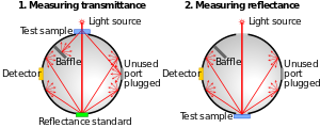
\includegraphics[width=.75\columnwidth]{Figures/IS.png}
\caption[Schematic of an Integrating Sphere]{Schematic of an integrating sphere.}
\label{fig:IS_apparatus}
\end{figure}

\begin{figure}[!ht]
\centering
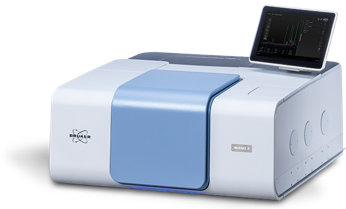
\includegraphics[width=.75\columnwidth]{Figures/FTIR.png}
\caption[Image of Fourier Transform Infrared Spectrometer (FTIR) Apparatus]{Image of Fourier transform infrared spectrometer (FTIR) apparatus.}
\label{fig:FTIR_apparatus}
\end{figure}

\subsubsection{Sample Preparation}

Specimens for the IS experiments were cut into 25~mm diameter cylindrical samples and the exposed surface of the sample was unchanged from the as-received state to ensure the optical properties were representative of the materials encountered in practice. 

\subsubsection{Calibration}

Prior to testing on a daily basis, the laser wavenumber was measured and calibrated to ensure accurate spectral data and a performance qualification (PQ) test was conducted to ensure the instrument was operating properly. The process for laser wavenumber calibration involved measuring a water vapor spectrum, determining the optimum wavenumber for a specific water band, and comparing against adjacent water bands. The calibrated laser wavenumber was verified against bands of a polystyrene internal validation unit filter in the final step of the calibration. The PQ test consisted of seven individual tests that ensured the FTIR signals were measured with the correct amplitude over the entire spectral range and that all optical components within the instrument were functioning properly. For all of these daily calibrations a gold reference material was in place at the lower measurement port when the IS was installed.

\subsubsection{Experimental Procedure}

The IS experiments consisted of a series of consecutive tests in which the spectral reflectance was measured for a reference standard, followed by a spectral reflectance measurement for the sample material. The reference standard used in these experiments was a light trap that represented the lowest possible reflectance that could be practically measured at all wavelengths. Tests were conducted with the liquid nitrogen-cooled MCT detector scanning at a rate of 40 kHz for a total of 256 scans per test. Eight replicates of the series which consisted of a reference test followed by a sample test were conducted for each material to collect statistics on the optical properties of the material.

When it was apparent that the sample material was non-opaque to the incident electromagnetic radiation in the infrared range, the transmittance through the material was also measured in IS experiments. For the transmission IS experiments, samples of several thicknesses of the material up to approximately 3~mm were prepared for testing. Each sample was mounted on a sample holder that held the sample at the entrance port to the IS such that the beam passed through the sample prior to entering the IS. Prior to the sample test, a reference test was conducted with no sample in the holder. Gold surface reference objects were placed at all other ports during these experiments. Eight replicates of the series of reference tests followed by sample tests were completed for each thickness of the material. These data were used to calculate the absorption coefficient of the material. 

\subsubsection{Experimental Uncertainty}

A comprehensive discussion of sources of uncertainty for integrating sphere reflectance measurements with the Bruker A562-G IS is provided by Blake et al.~\cite{Blake_2018}. To summarize the discussion, sources of systematic uncertainty include deviations from ideal geometry of the sphere and the sample that are not accounted for in theory and analysis. These deviations include a lack of knife edges at the interface between the IS and the sample, the use of a flat sample instead of a sample with the same curvature as the sphere, the detector field-of-view (FOV) and baffle position, and general FTIR baseline drift. Blake et al. conducted a ray trace analysis on an accurate three-dimensional model of the IS and determined the fractional uncertainties of each systematic contribution are those presented in Table~\ref{tab:IS_uncertainty}. The total uncertainty due to these systematic components is approximately $\pm$4\%. These components must be added in quadrature with the aleatoric uncertainty to get the total expanded uncertainty in the spectral reflectance measurements.

\begin{table}[!ht]{}
\centering
\caption[Components of Systematic Uncertainty in Integrating Sphere Experiments]{Components of Systematic Uncertainty in Integrating Sphere Experiments (Reproduced from~\cite{Blake_2018})}
{\begin{tabular}{cc}
\toprule
Component                         & Fractional Uncertainty  \\
\midrule
Effect of port edges (no knife edge)        & 0.03 					    \\ 
Effect of flat sample                       & 0.002                       \\ 
Effect of detector FOV and baffle position  & 0.008                       \\ 
FTIR baseline drift                         & 0.002                       \\ 
\bottomrule
\end{tabular}}
\label{tab:IS_uncertainty}
\end{table}

\subsection{Cone Calorimeter}
\label{sec:cone_calorimeter}

The cone calorimeter, pictured in Figure~\ref{fig:cone} is a standard test apparatus~\cite{ASTM_E1354} that utilizes oxygen consumption calorimetry to provide data on the HRRPUA of a sample material subjected to a well-defined external heat flux and under flaming conditions. The cone calorimeter features a truncated conical heater with the bottom surface parallel to and 25~mm above the surface of a 0.1~m square sample. The standard test features a spark igniter that ignites gaseous pyrolyzate when the concentration of gases 13~mm from the surface of the sample exceed the lower flammability limit. The mass of the sample is measured through the duration of the test and the gaseous effluent is pulled into a ventilation system at a well-defined flow rate. A gas sampling system measures the reduction in oxygen and increase in carbon dioxide and carbon monoxide from baseline conditions over the duration of the test. A laser system also measures the optical density of the effluent throughout the duration of the test, which can be directly related to the specific extinction area and smoke yield per mass of sample lost.

\begin{figure}[!ht]
\centering
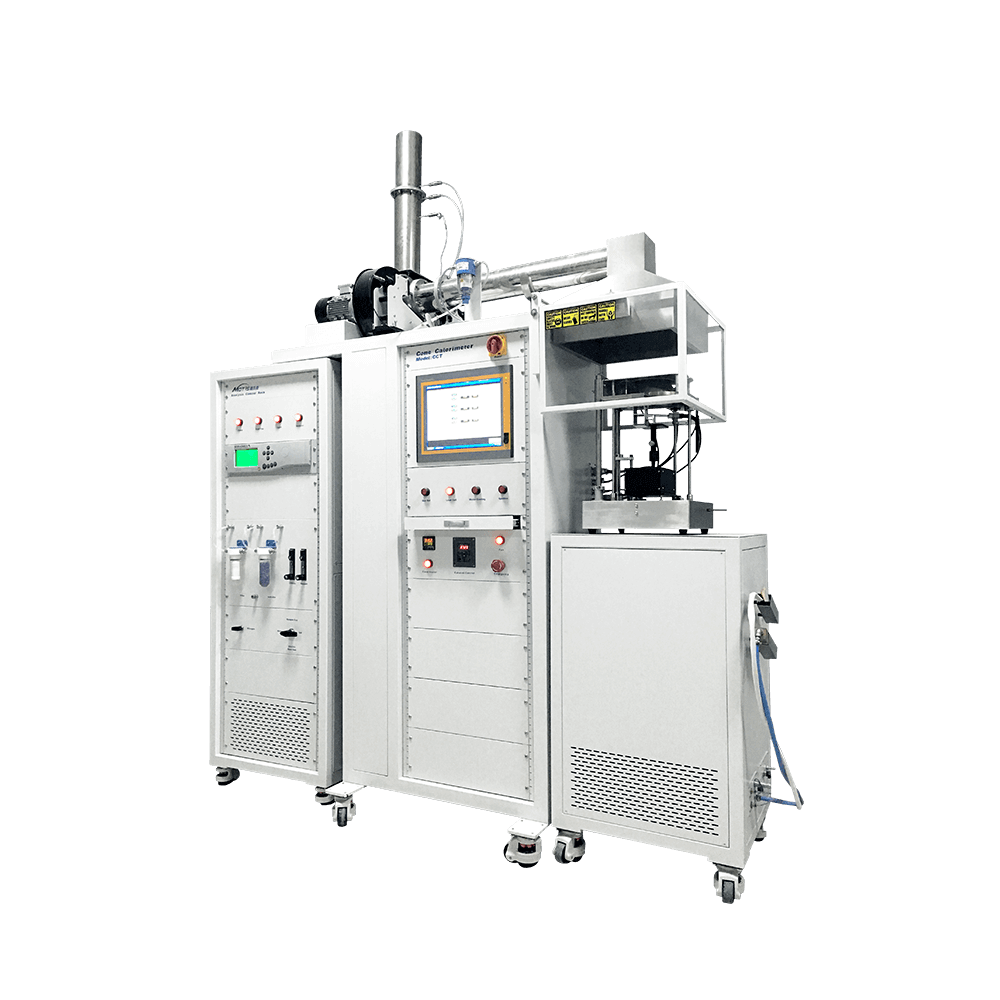
\includegraphics[width=.75\columnwidth]{Figures/Cone.png}
\caption[Image of Cone Calorimeter]{Image of cone calorimeter.}
\label{fig:cone}
\end{figure}

\subsubsection{Sample Preparation}

Samples were cut into 0.1~m x 0.1~m specimens and stored in a conditioning chamber at 50\% RH and \degC{23}. The mass and dimensions of the sample specimens were recorded and pictures were taken of the specimens prior to testing. Pictures were also taken after the tests to provide context for the collected data. The edges of the sample specimens were wrapped with aluminum foil such that only the top surface was exposed. The sample specimen was placed on a minimum of 0.025~m thick refractory blanket insulation. Every effort was made to avoid the use of the edge frame and the retaining grid to limit unnecessary thermal mass that is difficult to represent in fire models. When samples deformed rapidly on exposure to the heater or intumesced significantly, relatively low mass tie wires were used to maintain the sample in place. When the tie wires were unable to keep the sample specimen in place, the retaining grid was used. When the retaining grid was required, the time to sustained ignition was verified against at least one test conducted without the retaining grid. Figure~\ref{fig:cone_sample} displays photographs of representative materials prepared for cone calorimeter tests.

\begin{figure}[H]
    \centering
    \begin{subfigure}[b]{0.475\textwidth}
        \centering
        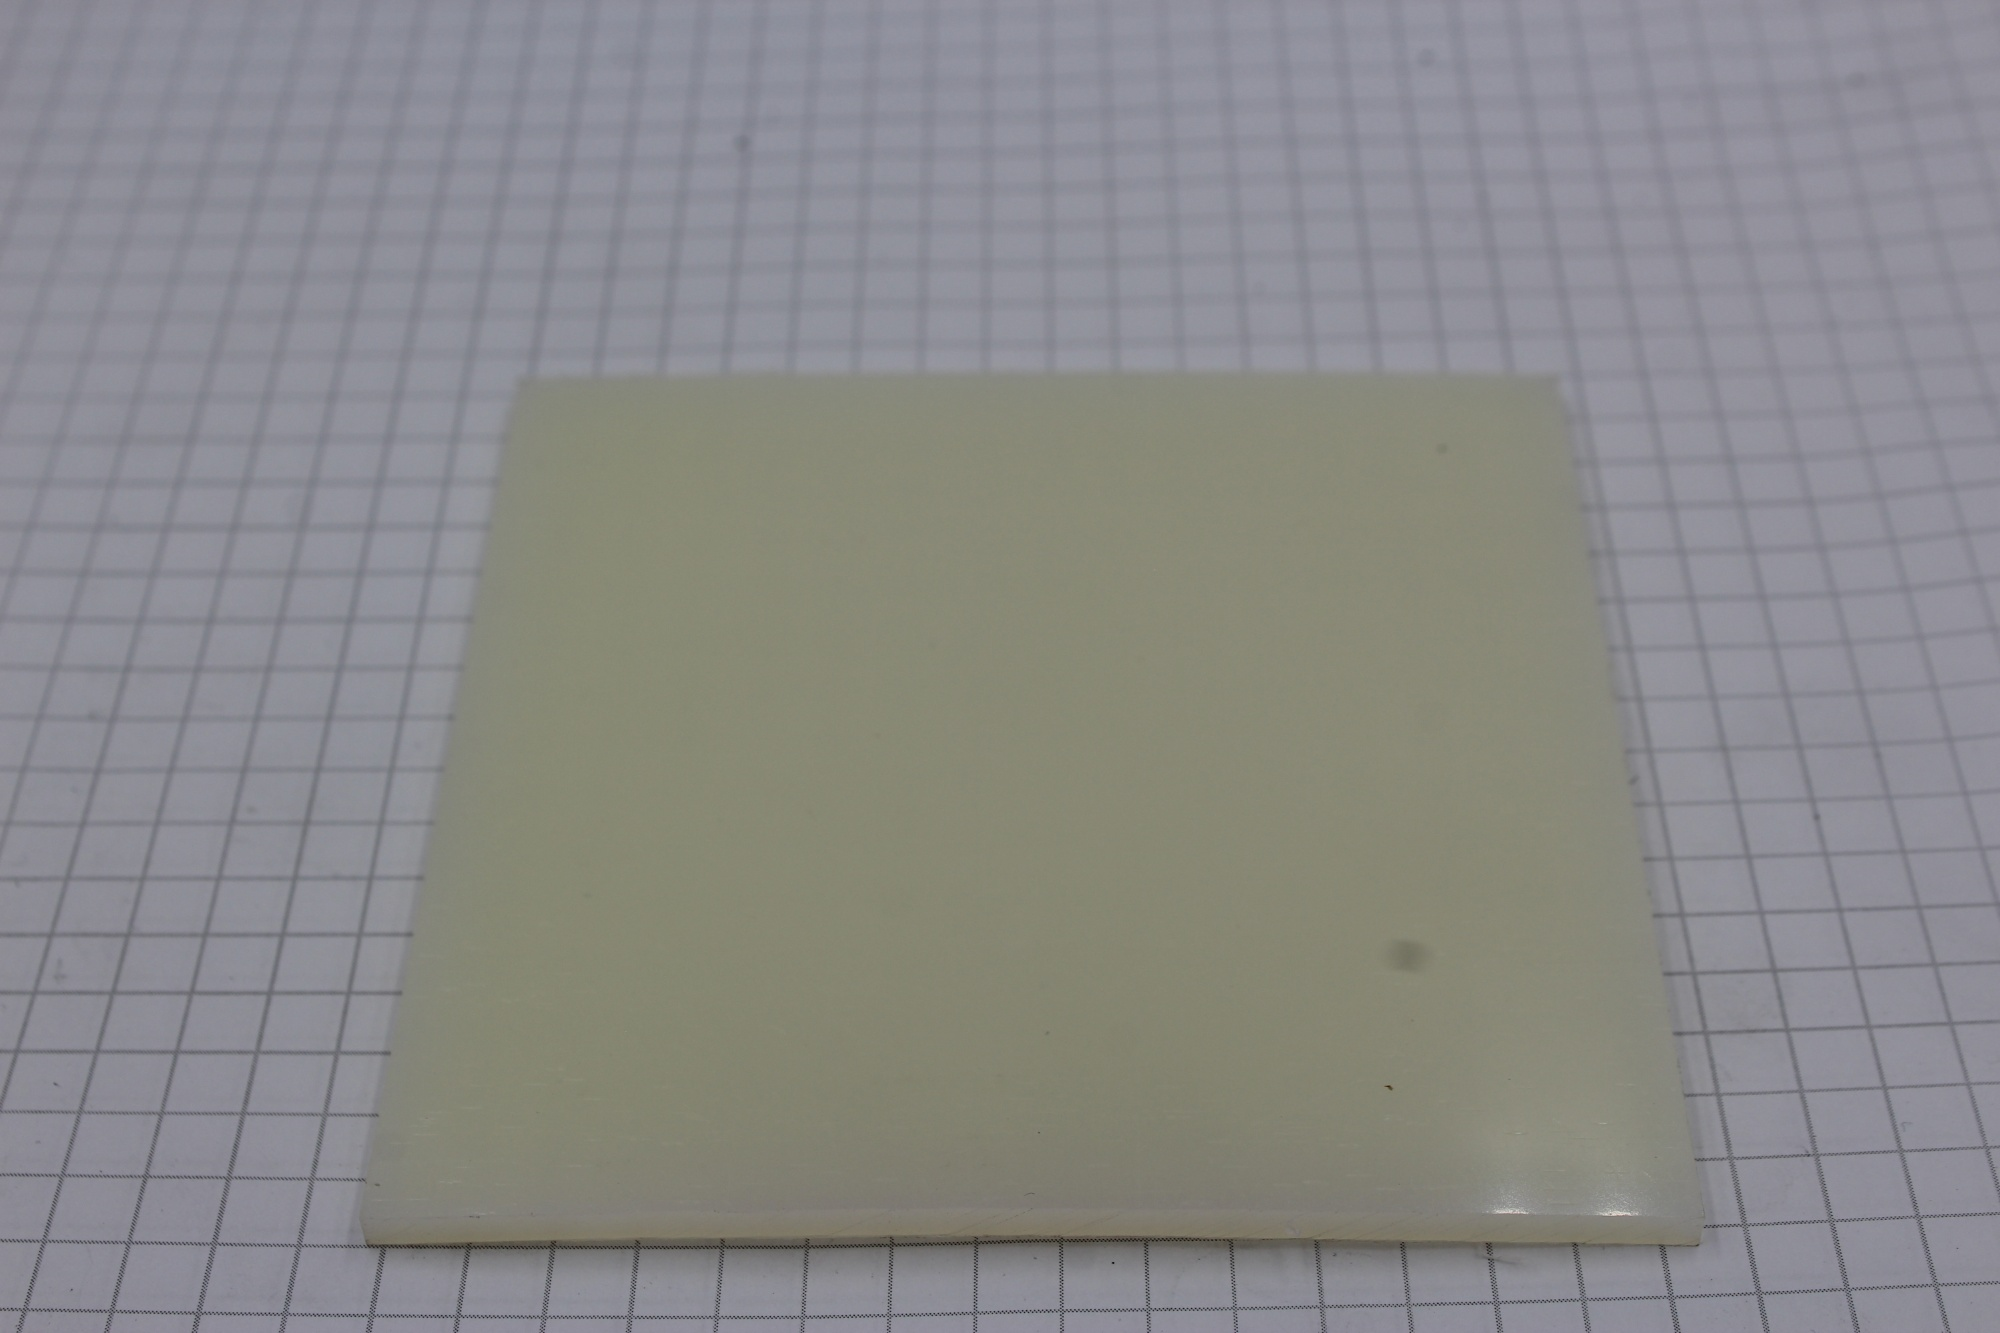
\includegraphics[width=\textwidth]{Figures/Nylon.jpg}
        \caption{Nylon sample prepared for cone calorimeter test}
    \end{subfigure}
    \hfill
    \begin{subfigure}[b]{0.475\textwidth}
        \centering
        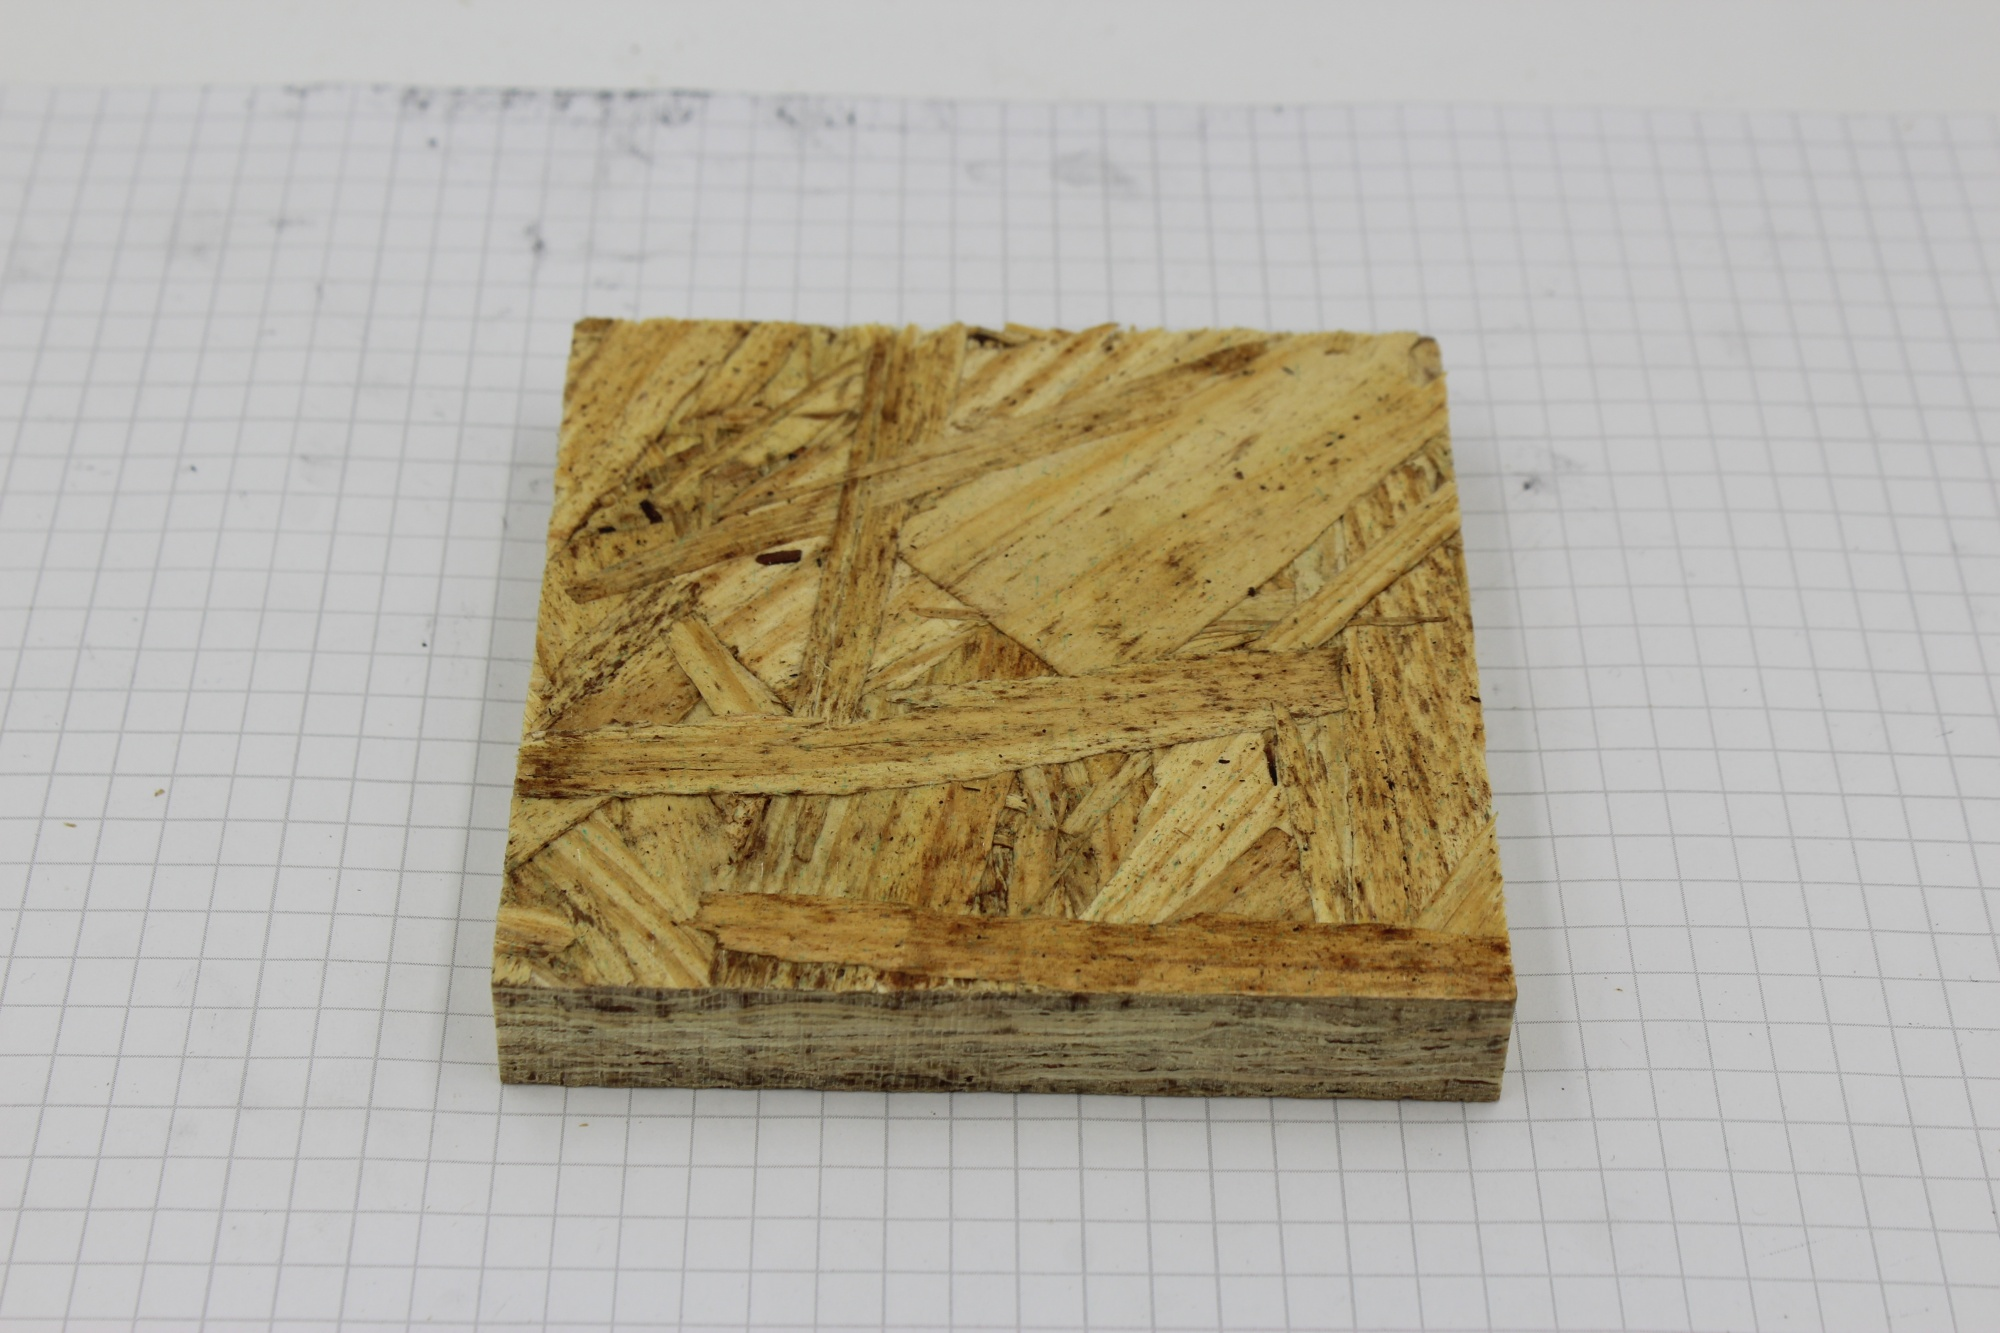
\includegraphics[width=\textwidth]{Figures/OSB.jpg}
        \caption{OSB sample prepared for cone calorimeter test}
    \end{subfigure}
    \caption[Representative Samples Prepared for Cone Calorimeter Experiments] {Representative samples prepared for cone calorimeter experiments.} 
    \label{fig:cone_sample}
\end{figure}

\subsubsection{Calibration}

The cone calorimeter was calibrated according to the standard calibration procedures~\cite{ASTM_E1354}. The oxygen, carbon dioxide, and carbon monoxide detectors were zeroed and calibrated daily against air and calibration span gas, respectively, prior to testing. The heat release rate measurement was calibrated using a methane burner that produced a 5~kW flame. The steady state reduction in oxygen while the burner had a flame was correlated with the known heat release rate to determine a C-factor coefficient that was applied when measuring HRR during tests on material samples. The load cell was zeroed and calibrated using a 0.5~kg mass. The zero value for the smoke obscuration measurement was verified daily prior to testing. The incident heat flux to the sample was set prior to each set of tests conducted at each heat flux through an automated algorithm that changed the temperature of the cone heater coil based on feedback from a Schmidt-Boelter heat flux gauge with the sensing surface flush with the exposed sample surface.

\subsubsection{Experimental Procedure}

Cone calorimeter tests were conducted in triplicate with incident heat fluxes of 25~kW/m$^2$, 50~kW/m$^2$, and 75~kW/m$^2$. The heater temperature was set using the feedback control algorithm with the signal from the Schmidt-Boelter heat flux gauge with the sensing surface at the same level as the sample. The data acquisition system was started and background data were collected. The sample specimen in the sample holder was placed on the mass balance platform and the mass measurement was tared for the initial mass of the sample holder and the specimen. Prior to the beginning of the test, a heat shield protected the sample surface from the heater. The spark igniter was moved into place 13~mm above the center of the sample surface and was energized. The heat shield was removed to begin the test, and the time at which the shield was removed was recorded. The sample specimen was observed throughout the test, and the engineer running the tests recorded the times at which offgassing started, flashing was observed, sustained ignition was observed, and the times at which any other pertinent phenomena were observed. The test was allowed to continue until the mass loss rate (MLR) or HRR dropped below a specific threshold, or was allowed to progress for a maximum of 20 minutes if ignition never occurred. 

\subsubsection{Experimental Uncertainty}

The sources of systematic uncertainty in the heat release rate determination with the cone calorimeter have been discussed by several researchers~\cite{Enright,Brohez,Zhao}. The most significant sources of uncertainty of measurement of HRR were identified as the assumed effective heat of combustion term, the combustion expansion factor, and uncertainty in the oxygen analyzer. The assumed effective heat of combustion may vary $\pm$5\%, the uncertainty in the combustion expansion factor is assumed to be approximately $\pm$33\%, and the absolute uncertainty in the oxygen concentration measurement is $\pm$100~ppm. The authors agree that uncertainty in the pressure transducer and temperature measurements associated with the HRR measurement are negligible relative to the other components of uncertainty. The total expanded relative uncertainty of the HRR measurement, when considering only the systematic contributions was estimated as between 5.5\% and 7\%~\cite{Enright,Zhao}. 

Additionally, the uncertainty in the measurement of mass with the balance was determined by Zhao and Dembsey~\cite{Zhao} to be approximately $\pm$0.38~g, and the authors remarked that this is lower than the uncertainty reported by the manufacturer ($\pm$0.5~g). The authors conducted an uncertainty analysis on the smoke meter system and found that the total expanded relative uncertainty of the main photodiode detector was $\pm$2.4\% and $\pm$0.8\% for the reference photodiode detector, but also stated that the smoke obscuration measurement system that was characterized was a custom-built system and may not provide a universal representation of all smoke obscuration systems.

The ASTM and ISO standards each report the results of interlaboratory studies on repeatability and reproducibility for the measurements made with the cone calorimeter. Linear regression coefficients for each metric are reported in the standards. The repeatability is defined as the deviation from a measured quantity that is expected with 95\% probability when tests are conducted under identical conditions on the same material in the same laboratory in rapid succession. The reproducibility is defined as the deviation from a measured quantity that is expected with 95\% probability when tests are conducted under identical conditions on the same material in a different laboratory. While these quantities do not provide direct quantifications of the components of systematic and aleatoric uncertainty, the repeatability provides an approximation of the aleatoric uncertainty and the reproducibility provides an approximation of the total expanded uncertainty. The repeatability and reproducibility of several quantities that describe features in the data collected in cone calorimeter experiments are presented in Table~\ref{tab:cone_r_and_r}~\cite{ASTM_E1354,ISO_5660-1}. Each value in the table is represented as a linear expression with a constant component and a component that is dependent on the magnitude of the quantity.

\begin{table}[!ht]{}
\centering
\caption[Kinetic Parameters Determined for Anaerobic Decomposition of Nylon]{Kinetic Parameters Determined for Anaerobic Decomposition of Nylon}
{\begin{tabular}{lcc}
\toprule
Quantity & Repeatability	& Reproducibility\\
\midrule
time to ignition ($t_{ig}$)			& $4.1 \pm 0.125t_{ig}$ 	& $7.4 \pm 0.220t_{ig}$	\\ 
peak HRR  ($\dot{q}''_{max}$)			& $13.3 \pm 0.131\dot{q}''_{max}$ 	& $60.4 \pm 0.141\dot{q}''_{max}$	\\ 
total heat released ($q''_{tot}$) 			& $7.4 \pm 0.068q''_{tot}$  	&	$11.8 \pm 0.088q''_{tot}$	\\ 
effective heat of combustion ($\Delta{h_{c,eff}}$) 			& $1.23 \pm 0.050\Delta{h_{c,eff}}$ 	&	$2.42 \pm 0.055\Delta{h_{c,eff}}$	\\ 
average specific extinction area ($\sigma_f$) 			& $59 \pm 0.076\sigma_f$	&	$63 \pm 0.215\sigma_f$	\\ 
\bottomrule
\end{tabular}}
\label{tab:cone_r_and_r}
\end{table}

\chapter{Data Analysis}
\label{sec:analysis}

User groups that are likely to use modeling methods that require similar properties were identified during this project to ensure all stakeholders were appropriately represented. Table~\ref{tab:user_group_properties} was reproduced from an earlier status report and presents the identified user groups and the properties that would be most useful for each group. The user groups include fire investigators, fire protection engineers, and fire researchers. The following sections describe how data were analyzed from the raw quantities measured in each of the experimental methods to yield the property values presented in the database as well as recommended methods for analyzing the data to extract property values when these values are not presented in the database. 

In each section, some example data is provided to illustrate the analytical methods and final results of analysis for sample materials. Sample materials included a thermoplastic, nylon (polyamide 6,6), and lignocellulosic materials, oriented strandboard (OSB) and masonite. Thermoplastics and lignocellulosic material typically have different trends in properties and reaction-to-fire test data and represent the range of methods required for analysis. Nylon is a non-charring (char fraction < 10\%) general polymer that is a common component in electronics and machine parts and is ubiquitous in the built environment. OSB is a wood-based material comprised of strands of softwood and a binder. OSB is a charring, lignocellulosic material that is used as sheathing in construction. Masonite is an engineered wood hardboard comprised of wood chips processed with steam and compressed into a high density board without additional adhesive.

Unless otherwise noted, all uncertainties presented in the following sections are associated with the repeatability of each measurement or calculated quantity. This is representative of the aleatoric or random uncertainty, and the total expanded uncertainty would require the aleatoric uncertainty to be added in quadrature with the systematic uncertainty which have been discussed in the previous sections. 

\begin{table}[!ht]
\centering
\caption[Expected Property Requirements for Each User Group]{Expected Property Requirements for Each User Group. (X indicates the user group is expected to use the property directly, and V indicates the user group is expected to user the property or data for validation purposes)}
	\begin{tabular}{rcccccccccccccccc}
		\toprule
		\textbf{User Group} & \rotatebox{90}{HRR} & \rotatebox{90}{Time to Ignition} & \rotatebox{90}{Ignition Temperature} & \rotatebox{90}{Soot Yield} & \rotatebox{90}{CO Yield} & \rotatebox{90}{Reaction Kinetics} & \rotatebox{90}{Melting Temperature} & \rotatebox{90}{Heat of Reaction} & \rotatebox{90}{Heat of Gasification} & \rotatebox{90}{Heat of Combustion} & \rotatebox{90}{Density} & \rotatebox{90}{Thermal Conductivity} & \rotatebox{90}{Specific Heat Capacity} & \rotatebox{90}{Emissivity} & \rotatebox{90}{Absorption Coefficient} & \rotatebox{90}{Radiative Fraction} \\
		\midrule
			Fire Investigators			& X	& X	& X & X	& 	& 	& X & 	&   & X	& X	& X	& X	& 	& 	& X \\ 
			Fire Protection Engineers	& X	& X	& X & X	& X	& X	&	&	& X & X	& X	& X	& X	& 	& 	& X \\ 
			Fire Researchers			& V	& V	& V & V	& X	& X	& X	& X	& X & X	& X	& X	& X	& X	& X	& X \\ 
		\bottomrule
	\end{tabular}
\label{tab:user_group_properties}
\end{table}

\section{Density}

Density was directly measured and no analysis was required to get a final value for density. Table~\ref{tab:density} displays the density of nylon and OSB measured in an unconditioned state and dried state. The nylon sample did not change mass during the drying process, which indicates it is not a hydrophilic material. OSB lost approximately 5\% of its mass during drying. This drying process had a marked effect on the specific heat capacity and thermal conductivity of the material. 

\begin{table}[!ht]{}
\centering
\caption[Density of Nylon and Masonite]{Density of Nylon and Masonite}
{\begin{tabular}{ccc}
\toprule
Material 				& Unconditioned [kg/m$^3$]	& Dried [kg/m$^3$] \\
\midrule
Nylon 					& 1070 $\pm$ 10				& 1070 $\pm$ 10 \\
Masonite				& 1130 $\pm$ 30				& 1070 $\pm$ 30  \\
\bottomrule
\end{tabular}}
\label{tab:density}
\end{table}

\section{Specific Heat Capacity}

The specific heat capacity was directly measured using the HFM. The maximum sample temperature that may be achieved when measuring specific heat capacity with the HFM is \degC{40}, which is not representative of materials exposed to fire-like temperatures. Table~\ref{tab:hfm_cp} presents the specific heat capacity measured with the HFM for nylon and OSB through the available temperature range. For both materials, the heat capacity increased with increasing temperature.

\begin{table}[!ht]{}
\centering
\caption[Thermal Conductivity of Nylon and Masonite]{Thermal Conductivity of Nylon and Masonite Measured with the HFM}
{\begin{tabular}{ccccc}
\toprule
Material 					& \degC{10} [J/g-K]		& \degC{20} [J/g-K]		& \degC{30} [J/g-K]	& \degC{40} [J/g-K]  \\
\midrule
Nylon (Unconditioned) 		& 1.52 $\pm$ 0.05		& 1.62 $\pm$ 0.06 		& 1.76 $\pm$ 0.08 	& 1.84 $\pm$ 0.08 \\
Masonite (Unconditioned) 	& 1.32 $\pm$ 0.07		& 1.39 $\pm$ 0.07 		& 1.46 $\pm$ 0.07 	& 1.52 $\pm$ 0.07 \\
Masonite (Dried) 			& 1.20 $\pm$ 0.07		& 1.25 $\pm$ 0.07 		& 1.30 $\pm$ 0.07 	& 1.35 $\pm$ 0.07 \\ 
\bottomrule
\end{tabular}}
\label{tab:hfm_cp}
\end{table}

Data from STA experiments may also be manipulated to calculate an apparent temperature-dependent specific heat capacity that is valid over a wider range of temperatures. The procedure for calculating the apparent specific heat capacity is a modification of the ASTM E1269 standard~\cite{ASTM_E1269} and it stems from the energy balance on a sample in an STA experiment. Equation~\ref{eq:thermal_analysis_heat_flow} is the representation of this energy balance. In the equation, $\dot{q}_{c}(T_s)$ is the heat flow rate to the sample with respect to the sample temperature [mW], $m_0$ is the initial mass of the sample [mg], $Y_{i}$ is the mass fraction of component $i$ [mg/mg], $C_{s,i}$ is the specific heat capacity of component $i$ [mg/mg], $H_j$ is the heat evolved in reaction $j$ [mJ/mg], and $H_m$ is a source term that represents the heat flow rate to the sample during melting [mW/mg]. The first term on the right hand side represents the sensible enthalpy. The second term on the right hand side represents the energy absorbed or released during reactions and is summed over $n$ reactions. The first two terms on the right hand side are summed over all $k$ components. The third term on the right hand side is summed over all $l$ melting processes.

\begin{equation}
\frac{\dot{q}_{c}(T_s)}{m_0} = \sum_{i=1}^{k} [Y_{i}(T_s)C_{s,i}(T_s)\frac{\partial{T_s}}{\partial{t}}(T_s)+\sum_{j=1}^{n}\frac{dY_{i}}{dt}(T_s)H_j] + \sum_{m=1}^{l} H_m(T_s) \label{eq:thermal_analysis_heat_flow}
\end{equation}

Apparent specific heat may be determined in temperature ranges when reactions and melting do not occur. Figure~\ref{fig:cp_full} displays the apparent specific heat capacity calculated from DSC data over the full temperature range of the experiment as well as the Normalized MLR over the full temperature range to aid in identification of temperature ranges where no mass loss or physical changes occurred. This simplification removes the second and third terms from the analysis and leaves the sensible enthalpy term on the right hand side. Dividing the measured normalized heat flow rate on the left hand side by the heating rate $\frac{\partial{T_s}}{\partial{t}}$ results in the sum of the product of mass fraction and specific heat capacity. For samples that may be represented as a single component prior to decomposition, the apparent specific heat capacity may be determined directly through this method.

\begin{figure}[H]
    \centering
    \begin{subfigure}[b]{0.475\textwidth}
        \centering
        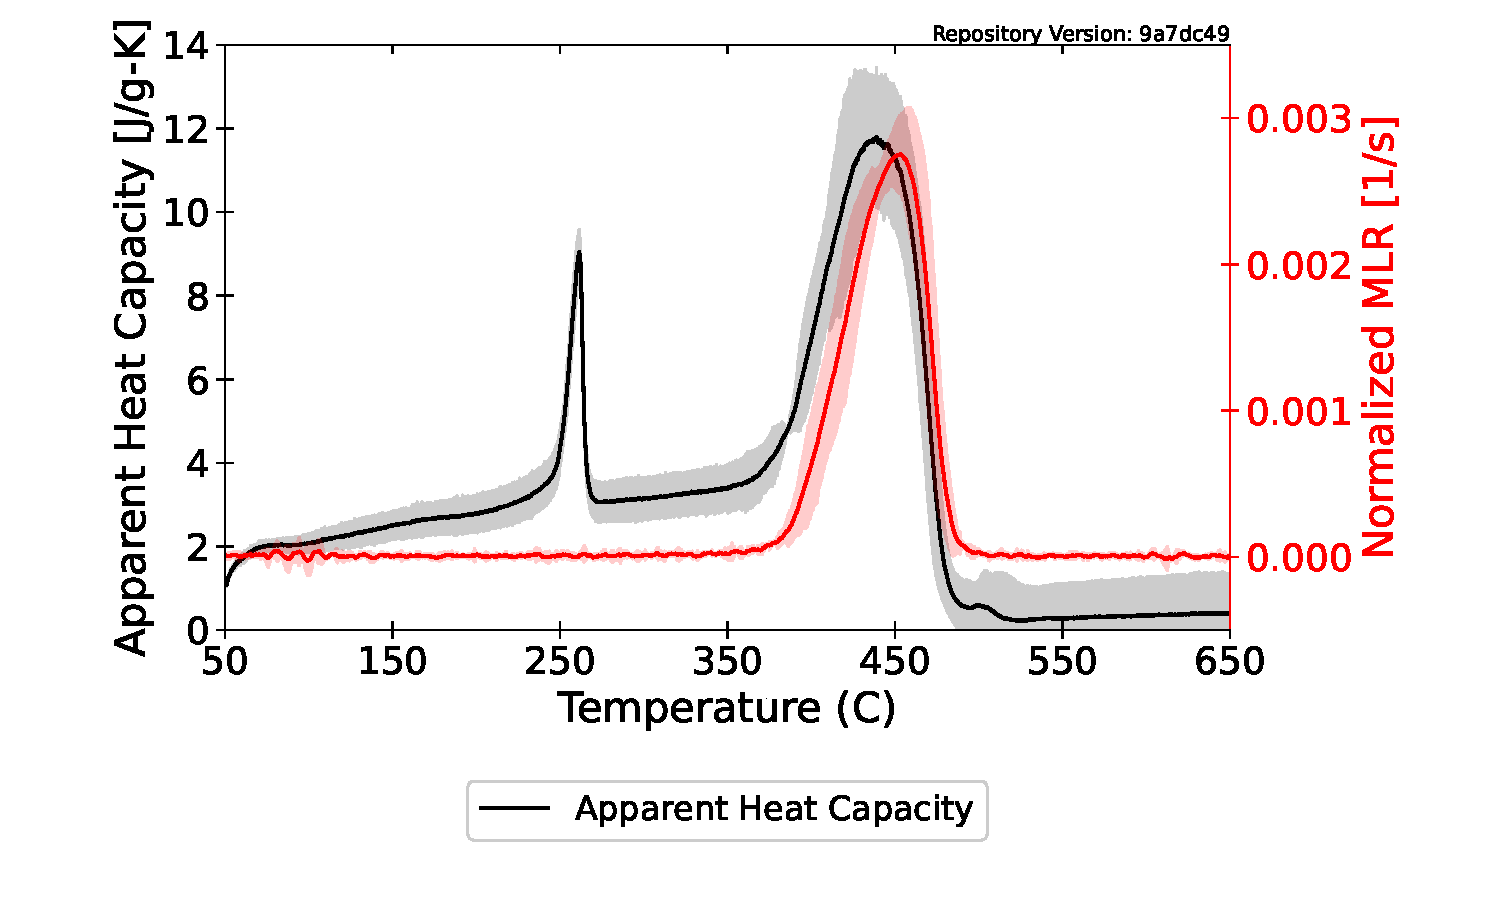
\includegraphics[width=\textwidth]{Figures/Nylon_10K_cp.pdf}
        \caption{Apparent specific heat capacity and Normalized MLR for nylon}
    \end{subfigure}
    \hfill
    \begin{subfigure}[b]{0.475\textwidth}
        \centering
        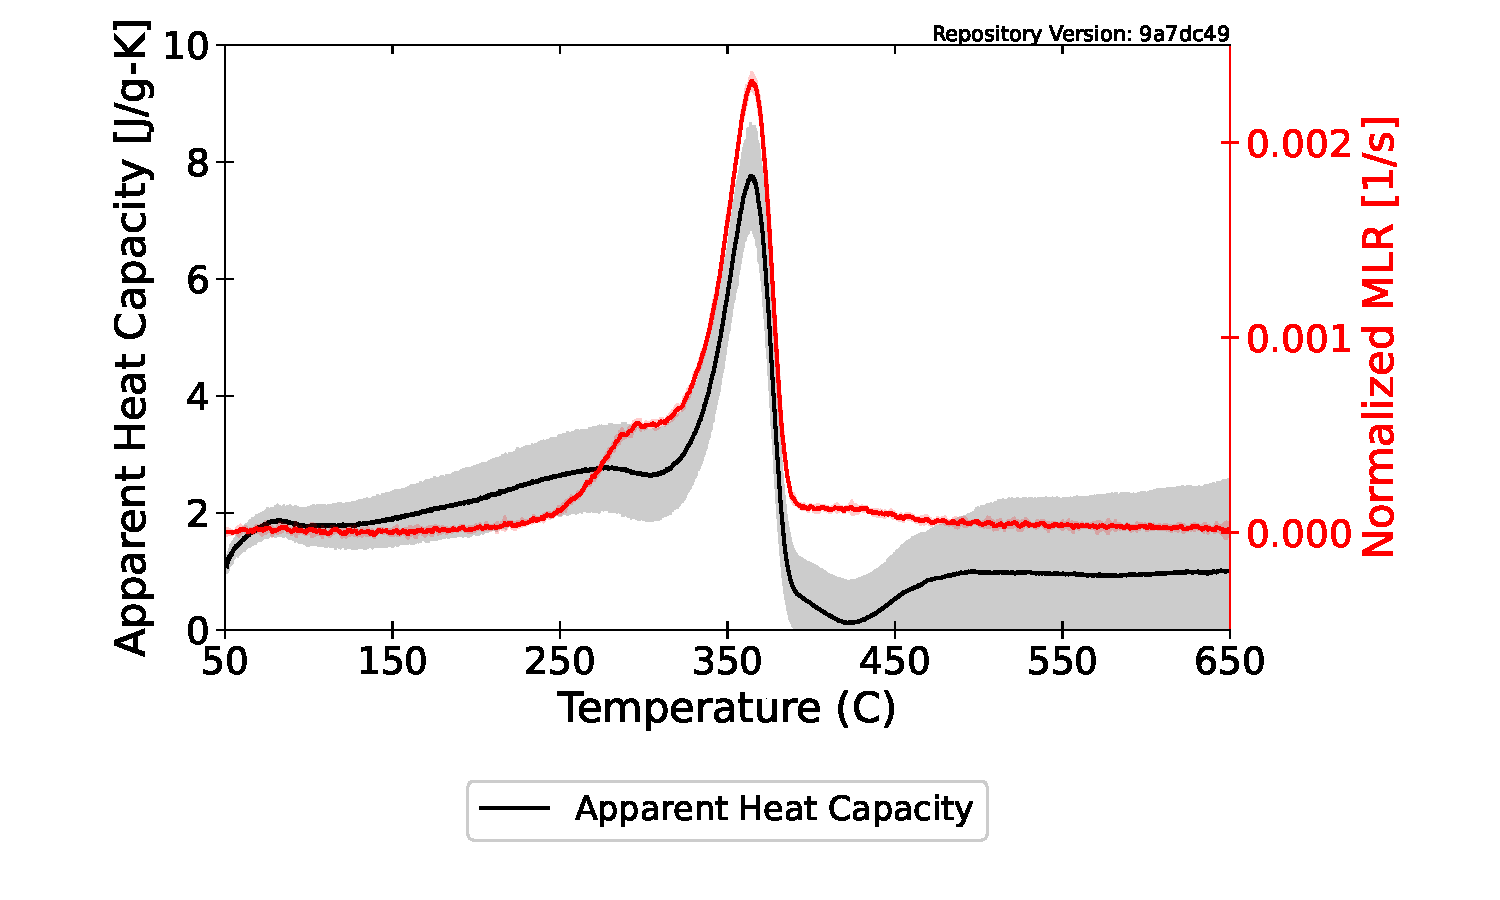
\includegraphics[width=\textwidth]{Figures/Masonite_Board_10K_cp.pdf}
        \caption{Apparent specific heat capacity and Normalized MLR for masonite}
    \end{subfigure}
    \caption[Apparent Specific Heat Capacity Plotted with Normalized MLR] {Apparent specific heat capacity plotted with Normalized MLR for nylon and masonite.} 
    \label{fig:cp_full}
\end{figure}

Figure~\ref{fig:cp_interval} displays the specific heat capacity measured with the HFM as well as the apparent specific heat capacity calculated from DSC data over temperature ranges where no mass loss occurred. By plotting the data from the DSC and the HFM on the same plot, regression can be conducted to determine a curve that best describes the specific heat capacity of the virgin material from room temperature to the onset of decomposition. Typically the line of best fit takes a linear form or that of a second-order quadratic, although other power law relationships have also been adopted in common pyrolysis models.

\begin{figure}[H]
    \centering
    \begin{subfigure}[b]{0.475\textwidth}
        \centering
        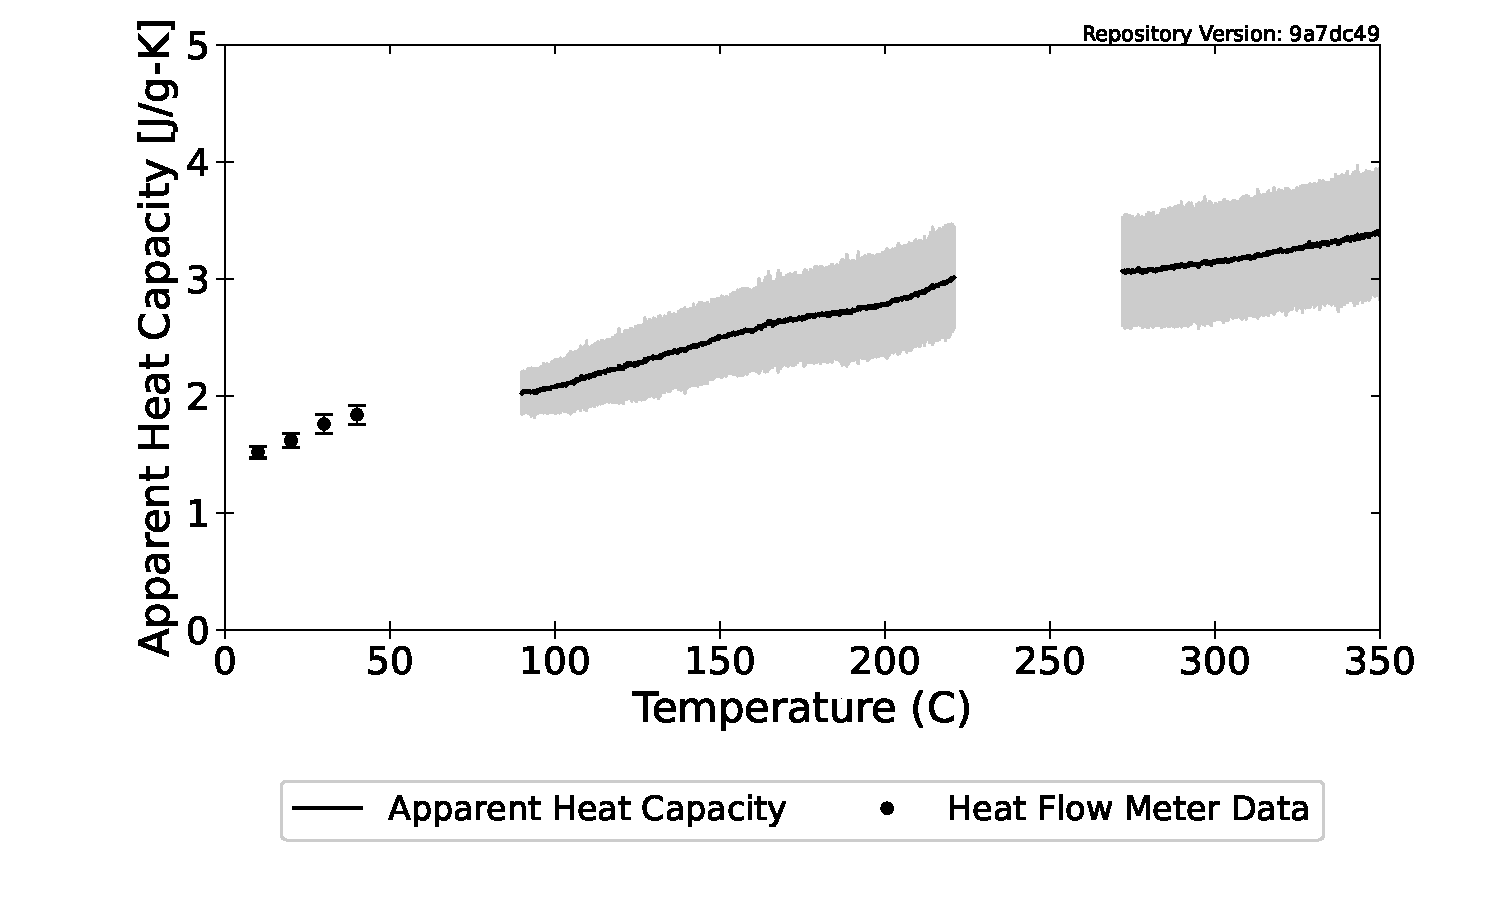
\includegraphics[width=\textwidth]{Figures/Nylon_10K_cp_interval_HFM.pdf}
        \caption{Specific heat capacity for nylon}
    \end{subfigure}
    \hfill
    \begin{subfigure}[b]{0.475\textwidth}
        \centering
        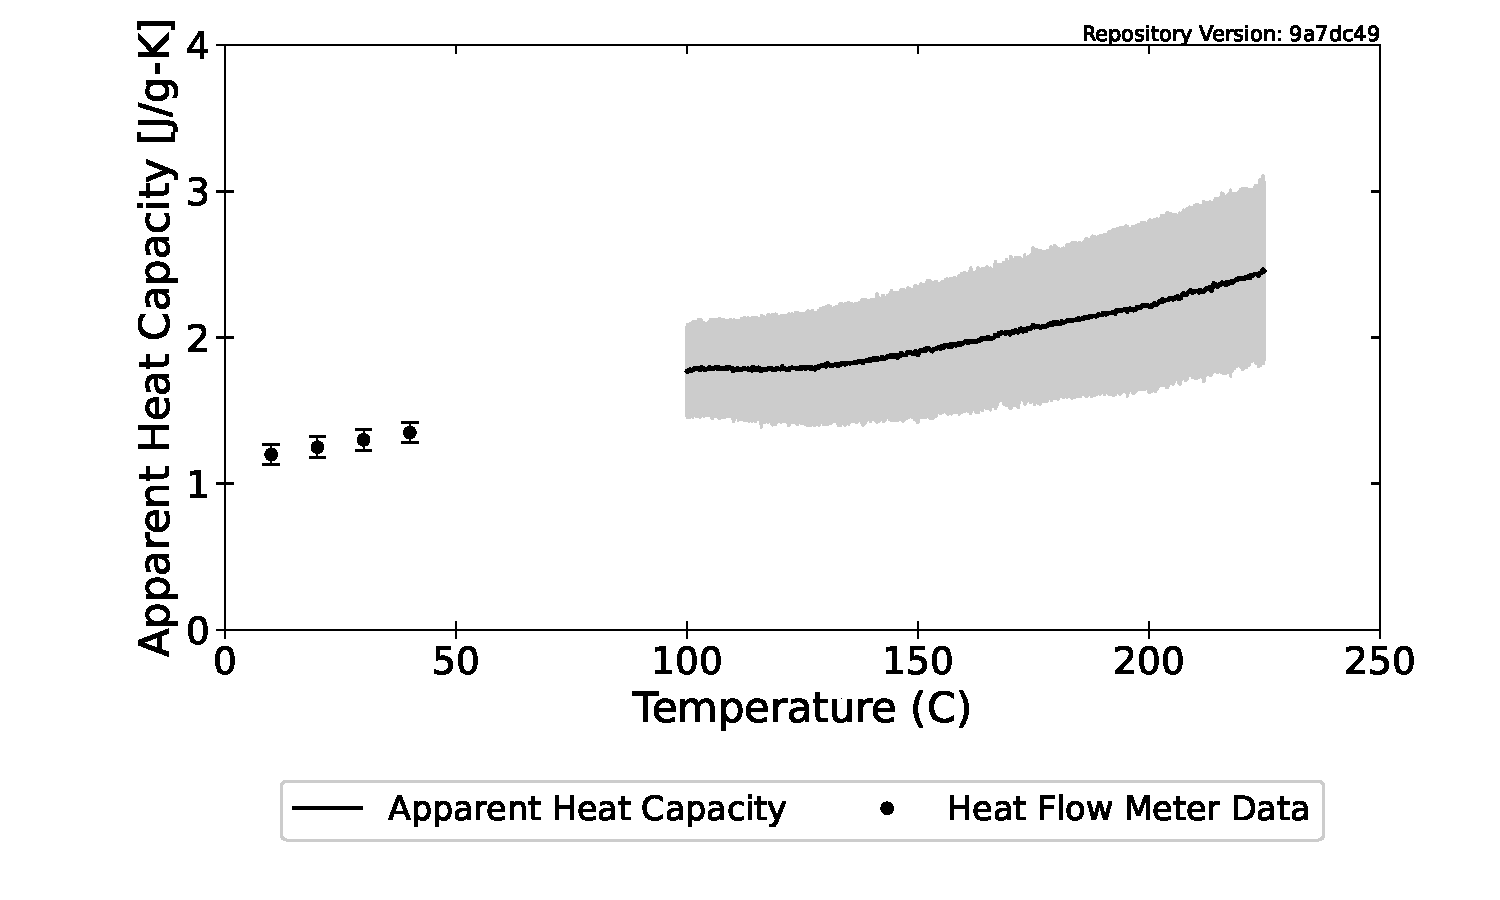
\includegraphics[width=\textwidth]{Figures/Masonite_Board_10K_cp_interval_HFM.pdf}
        \caption{Specific heat capacity for masonite}
    \end{subfigure}
    \caption[Temperature-Dependent Specific Heat Capacity] {Temperature-dependent specific heat capacity.} 
    \label{fig:cp_interval}
\end{figure}

\section{Reaction Kinetics}

The most common method in fire modeling to describe the temperature-dependence of the mass loss rate of a material is by adopting the definition of the reaction rate from chemistry. Chemical reaction rates are typically described using the Arrhenius equation. Equation~\ref{eq:arrhenius_rate} presents the general form of the reaction rate equation that is (or a modified form of which is) commonly invoked in pyrolysis models to describe the evolution of the composition of the material and its production of gaseous volatiles. The equation describes the the $j$th reaction that involves the $i$th reactant. The Arrhenius reaction parameters, which include the Arrhenius pre-exponential factor ($A_{ij}$) and the activation energy ($E_{ij}$), must be defined for the $j$th reaction. In addition to these parameters, a function of the instantaneous concentration of component $i$ (volumetric fraction, $X_{s,i}$ in the general equation) is multiplied by the temperature-dependent rate defined with the other parameters. The form of this function of concentration is commonly chosen as first order (concentration is multiplied directly with the rate), $n$th order (concentration is taken to a constant power and multiplied directly with the rate), or some other form representative of a specific phenomenon when it is known to occur. In the general form of the reaction rate, the volumetric concentration of oxygen in the vicinity of the reacting material may also modify the reaction rate. The concentration of oxygen $X_{O_2}$ is taken to a power of $n_{O_2,ij}$ to accelerate or decelerate the reaction rate. 

\begin{equation}
r_{ij} = A_{ij}\exp\left(-\frac{E_{ij}}{RT_s}\right)f(X_{i})X_{O_2}^{n_{O_2,ij}}\label{eq:arrhenius_rate}
\end{equation}

In the present form of the database, oxidative pyrolysis and oxidation have not been extensively studied or quantified and all thermal analysis data were collected in a nitrogen atmosphere, which takes the volumetric oxygen concentration to zero in Equation~\ref{eq:arrhenius_rate}. It was also assumed that all reactions were of the first order. This eliminated the need to determine the reaction order without significantly affecting the curves generated with the kinetic parameters. The default reaction scheme for all materials involved sequential reactions where a single solid reactant was typically converted to a single solid product and a single gaseous product as shown in Equation~\ref{eq:reaction_eqn} where $\nu_i',j$ is the stoichiometric coefficient for solid product i' in reaction $j$. In this scheme, the solid product of the first reaction is designated as the reactant in the following reaction, and so on until the final solid product does not participate in further reactions. 

\begin{equation}
\textrm{Reactant}_{i} \to \sum_{j=1}^{N_p}\nu_{i',j} \textrm{Solid Product}_{i'} + (1-\nu_{i',j}) \textrm{Gaseous Product}_{i''} \label{eq:reaction_eqn}
\end{equation}

There is no single, universally accepted, standard method in the fire modeling community to determine reaction kinetics, which can lead to a disparity between kinetic parameters determined by different investigators using disparate experimental and analytical methods. Part of the argument for defining pyrolysis kinetics in fire modeling is that definition of kinetics effectively decouples the mathematical description of burning from the experimental method, ignition source, or fuel configuration. Kinetics allow the model to be truly predictive by representing the burning rate as a function of temperature only.

There are many model-free methods (i.e. the form of the the function $f(X_{i})$ in Equation~\ref{eq:arrhenius_rate} is not assumed a priori) that require thermal analysis data collected at several heating rates. Some of these methods are described by ASTM E698 (Ozawa)~\cite{ASTM_E698}, ASTM E2890 (Kissinger)~\cite{ASTM_E2890}, and Friedman~\cite{Friedman}. These methods have been postulated as advantageous because the kinetics determined through isoconversional methods are informed by data collected at several heating rates and may be universally applicable over a wider range of conditions than kinetics determined from data collected at a single heating rate. Disadvantages of the model-free methods include that the typically do not yield a single, constant activation energy, which makes the results of little use in modern fire and pyrolysis models, and, because of this, they may only be sensible for single reaction mechanisms. 

Model-based methods typically require the practitioner to define a form of the kinetic model to describe the global reaction mechanism. There are no standard model-based methods and the majority of available methods rely on regression algorithms, optimization algorithms, or otherwise minimization of error between experimental data and model predictions. Some model-based methods have been described by Lautenberger~\cite{Lautenberger:2006,Lautenberger_2011}, Bruns and Leventon~\cite{Bruns_2021} and Fiola et al.~\cite{Fiola_2021}. Lautenberger was one of the first researchers to apply direct search optimization algorithms (e.g. genetic algorithm, shuffled-complex evolution, etc.) to property determination for fire models. The method described by Fiola et al. utilized a stochastic hill climber optimization algorithm to maximize a modified form of the coefficient of determination for a given data set. The analytical method described by Bruns and Leventon involved an approximate solution to the Arrhenius rate equation which utilized three different methods to estimate the peak temperature and the width of the peak. 

McKinnon et al. described an analysis whereby reaction kinetics parameters determined through several model-free and model-based methods may be displayed on a Constable plot of activation energy vs. the logarithm of the Arrhenius pre-exponential factor~\cite{McKinnon_ASTM}. This allowed for propagation of the uncertainty in the relationship between the kinetics parameters to the results of larger scale models. An approach similar to the one described by McKinnon et al. has been adopted for the database. In this approach, a nonlinear least squares (NLLS) algorithm is used to minimize the residuals between a predicted curve described by sequential first order reactions and the experimental data. TGA data from each experiment conducted at heating rates of 3, 10, and 30 K/min were analyzed individually with the NLLS algorithm as well as considering all datasets equally weighted in an objective function. When it was suspected that only single reaction was present, the kinetics were determined using model-free and model-based methods, whereas for materials described by multi-reaction schemes, only model-based methods where used.

Kinetics pairings for nylon and masonite are presented in Figure~\ref{fig:kinetics}, the kinetic parameters determined through each method for nylon are presented in Table~\ref{tab:nylon_kinetics} and for masonite in Table~\ref{tab:masonite_kinetics}. For all reactions, the plotted data are highly linear, which is a manifestation of the well-known kinetic compensation effect~\cite{KOGA_1994,Barrie_2012}. Because of the linearity between the activation energy and logarithm of the pre-exponential factor, pyrolysis model predictions are likely not highly sensitive to the method used to determine the pyrolysis kinetics. In theory, when defining a single set of kinetics in a model, any value along the line that best fits the kinetic pairs may be used to describe the temperature dependence of mass loss. Because of the strong linear relationship between the activation energy and the pre-exponential factor, when representing the uncertainty in the kinetic parameters, care must be to ensure the two parameters remain coupled and the relationship is adequately communicated.

\begin{figure}[H]
    \centering
    \begin{subfigure}[b]{0.475\textwidth}
        \centering
        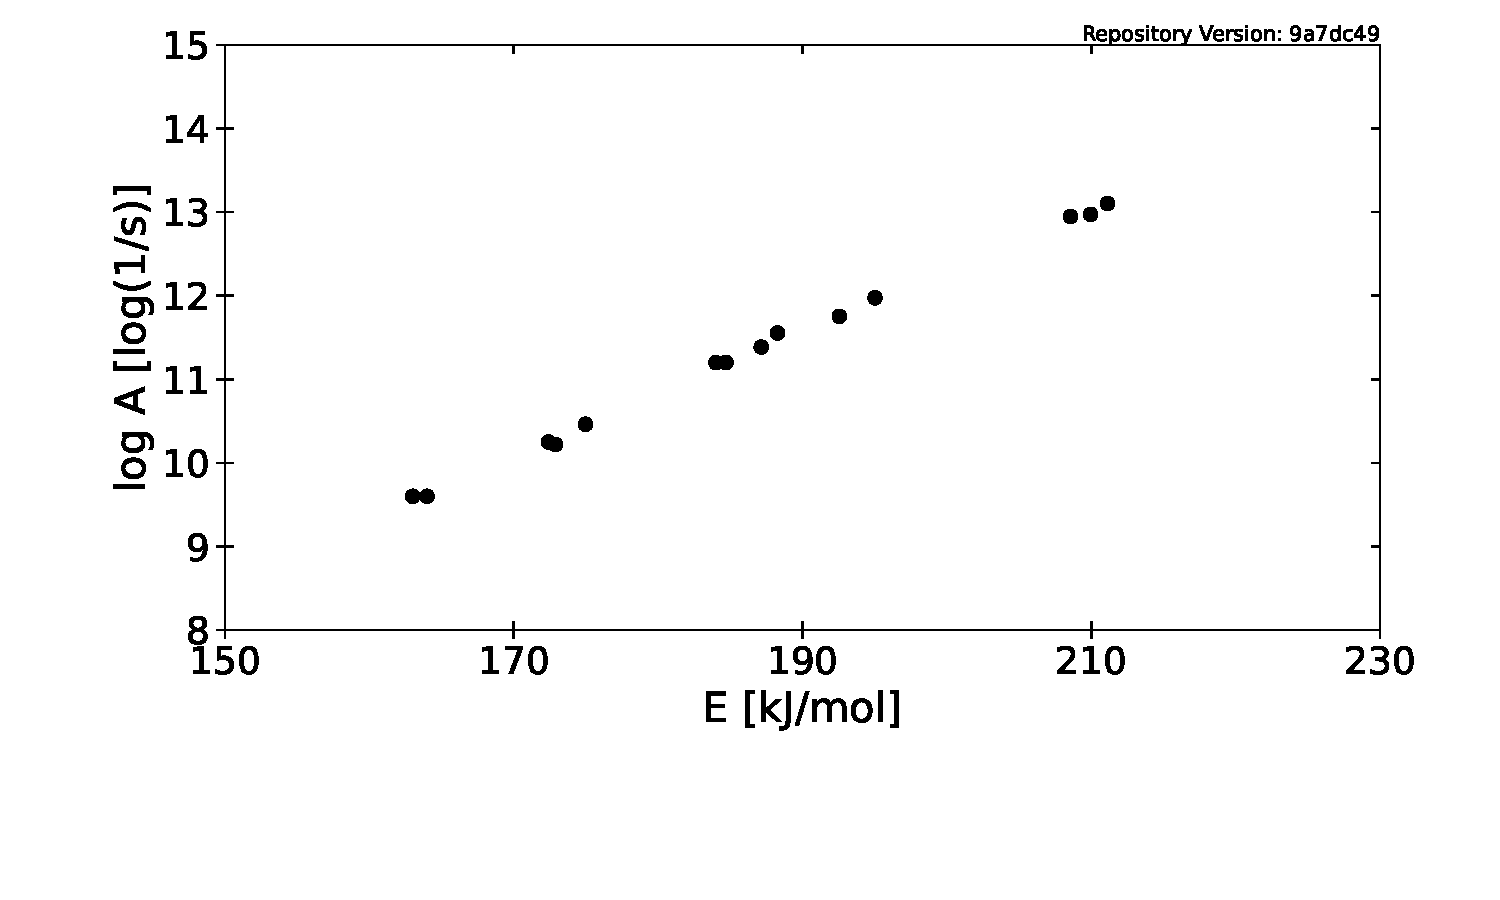
\includegraphics[width=\textwidth]{Figures/Nylon_kinetics.pdf}
        \caption{Kinetic parameters determined for nylon using model-free and model-based analytical methods}
    \end{subfigure}
    \hfill
    \begin{subfigure}[b]{0.475\textwidth}
        \centering
        \includegraphics[width=\textwidth]{Figures/Masonite_board_kinetics.pdf}
        \caption{Kinetic parameters determined for masonite using model-based analytical methods}
    \end{subfigure}
    \caption[Kinetic Parameters Determined for Nylon and Masonite] {Kinetic parameters determined for nylon and masonite.} 
    \label{fig:kinetics}
\end{figure}

For materials that can be easily described by a single reaction mechanism, and for materials that must be described by a multi-reaction scheme, kinetics determined through a model-based method are presented.

\begin{table}[!ht]{}
\centering
\caption[Kinetic Parameters Determined for Anaerobic Decomposition of Nylon]{Kinetic Parameters Determined for Anaerobic Decomposition of Nylon}
{\begin{tabular}{ccccc}
\toprule
E [kJ/mol] 		& log(A) [log(1/s)]  	& Char Fraction 	&  Method  & Dataset \\
\midrule
195.0 & 11.97 	& 	0.038	& NLLS  		& 10K/min (R1)  \\ 
192.6 & 11.75 	&	0.044	& NLLS  		& 10K/min (R2)  \\ 
188.3 & 11.56 	&	0.047	& NLLS 	 		& 10K/min (R3)  \\ 
211.1 & 13.10 	&	0.030	& NLLS  		& 30K/min (R1)  \\ 
210.0 & 12.97 	&	0.033	& NLLS  		& 30K/min (R2)  \\ 
208.6 & 12.95 	&	0.029	& NLLS  		& 30K/min (R3)  \\ 
175.0 & 10.46 	&	0.050	& NLLS  		& 3K/min (R1) \\ 
187.1 & 11.39 	&	0.039	& NLLS  		& ALL \\ 
164.0 & 9.6   	&	0.039	& ASTM E698~\cite{ASTM_E698} 		& ALL \\ 
163.0 & 9.6 	&	0.039	& ASTM E2890~\cite{ASTM_E2890}  		& ALL \\ 
184.0 & 11.2 	&	0.039	& Friedman~\cite{Friedman}  		& ALL \\ 
172.9 & 10.22 	&	0.039	& Ozawa-Flynn-Wall 					& ALL \\ 
172.4 & 10.25 	&	0.039	& Kissinger-Akahira-Sunose	 		& ALL \\ 
\bottomrule
\end{tabular}}
\label{tab:nylon_kinetics}
\end{table}

\begin{table}[!ht]{}
\centering
\caption[Kinetic Parameters Determined for Anaerobic Decomposition of Masonite]{Kinetic Parameters Determined for Anaerobic Decomposition of Masonite (subscripts indicate the reaction number)}
\resizebox{\textwidth}{!}{\begin{tabular}{ccccccccccc}
\toprule
$E_1$ [kJ/mol] & $\log(A_1)$ [log(1/s)]  & $\nu_1$ & $E_2$ [kJ/mol] & $\log(A_2)$ [log(1/s)]  & $\nu_2$ & $E_3$ [kJ/mol] & $\log(A_3)$ [log(1/s)]  & $\nu_3$ & Char Fraction & Dataset  \\
\midrule
96.7	&	6.47	&	0.817	&	191.9	&	13.81	&	0.371	&	14.4	&	-2.31	&	0.634	&	0.192	& 10K/min (R1)  \\ 
98.8	&	6.84	&	0.823	&	202.4	&	14.70	&	0.379	&	37.5	&	0.00	&	0.712	&	0.220	& 10K/min (R2)  \\ 
100.9	&	7.08	&	0.819	&	196.5	&	14.18	&	0.364	&	22.8	&	-1.13	&	0.682	&	0.203	& 10K/min (R3)  \\ 
102.3	&	7.20	&	0.820	&	193.2	&	13.90	&	0.369	&	25.4	&	-0.95	&	0.685	&	0.207	& 30K/min (R1)  \\ 
107.7	&	7.80	&	0.825	&	203.5	&	14.70	&	0.393	&	26.9	&	-0.36	&	0.716	&	0.230	& 30K/min (R2)  \\ 
102.6	&	7.34	&	0.822	&	200.5	&	14.46	&	0.385	&	24.5	&	-0.53	&	0.695	&	0.218	& 30K/min (R3)  \\ 
102.2	&	7.31	&	0.823	&	200.8	&	14.48	&	0.389	&	24.3	&	-0.54	&	0.697	&	0.221	& 3K/min (R1) \\ 
107.8	&	7.73	&	0.819	&	185.6	&	13.23	&	0.364	&	38.3	&	0.00	&	0.683	&	0.200	& ALL \\ 
\bottomrule
\end{tabular}}
\label{tab:masonite_kinetics}
\end{table}

\section{Melting Temperature}

STA data may be used to determine the temperature at which materials undergo physical transitions including melting and glass transition. By plotting mass loss rate (MLR) data on the same axes as heat flow rate data, the temperature ranges at which energetic physical transitions which correspond to no mass loss occur may be identified. 

Glass transition typically manifests as a step shift of the heat flow rate data. The glass transition temperature is determined by drawing a baseline consistent with the trend in the heat flow rate data before and after the transition. The glass transition temperature is defined as the mean of the temperatures at which the heat flow rate curve intersects each of the baseline curves. This analytical procedure is described in ASTM E1356~\cite{ASTM_E1356} and ISO 11357-2~\cite{ISO_11357-2}. This physical transition manifests as a change in the heat capacity and mechanical properties. It typically occurs at a relatively low temperature ($<$\degC{150}), and has a minimal affect on the overall pyrolysis process. The glass transition temperature was not determined for the materials presented in the database.

Melting manifests in heat flow rate data as an endothermic curve that increases from the baseline, reaches a peak, and decreases back to the baseline. This peak is not accompanied by a change in mass. Analysis is similar to determination of glass transition temperatures, except there is a single baseline. The temperature at which the heat flow rate curve deviates from the baseline is considered the onset temperature for melting and the temperature at which the maximum endothermic heat flow is measured is considered the peak melting temperature. Both quantities are typically reported as a result of this analysis and have been provided in the database for the materials which undergo melting. The area between the melting peak curve and the heat flow rate baseline is considered the enthalpy of fusion (enthalpy of melting). This analytical procedure is described in ASTM E793~\cite{ASTM_E793}, ASTM E794~\cite{ASTM_E794}, and ISO 11357-3~\cite{ISO_11357-3}.

The procedure for determining the peak melting temperature, the temperature at onset of melting, and the limits of integration to determine the enthalpy of melting for the values presented in the database is a multi-step process that begins with identification of the temperature at the melting peak. The temperature at the peak was determined by finding the roots of the derivative of the heat flow rate curve with respect to temperature. After identifying the peak melting temperature, a \degC{150} window centered at the peak melting temperature was extracted from the heat flow rate data and an iterative polynomial fit algorithm was used with a third-degree polynomial to automatically draw the baseline for the extracted data. The process involved iteratively performing polynomial regression and truncating all values in the data above the regression line, which eventually eliminated the peaks and left only the baseline. An example baseline drawn for nylon is provided in Figure~\ref{fig:nylon_melting}. The figure also shows the Normalized MLR curve collected at 10 K/min to illustrate that the energetic peak was not associated with a change in mass.

\begin{figure}[H]
    \centering
    \begin{subfigure}[b]{0.475\textwidth}
        \centering
        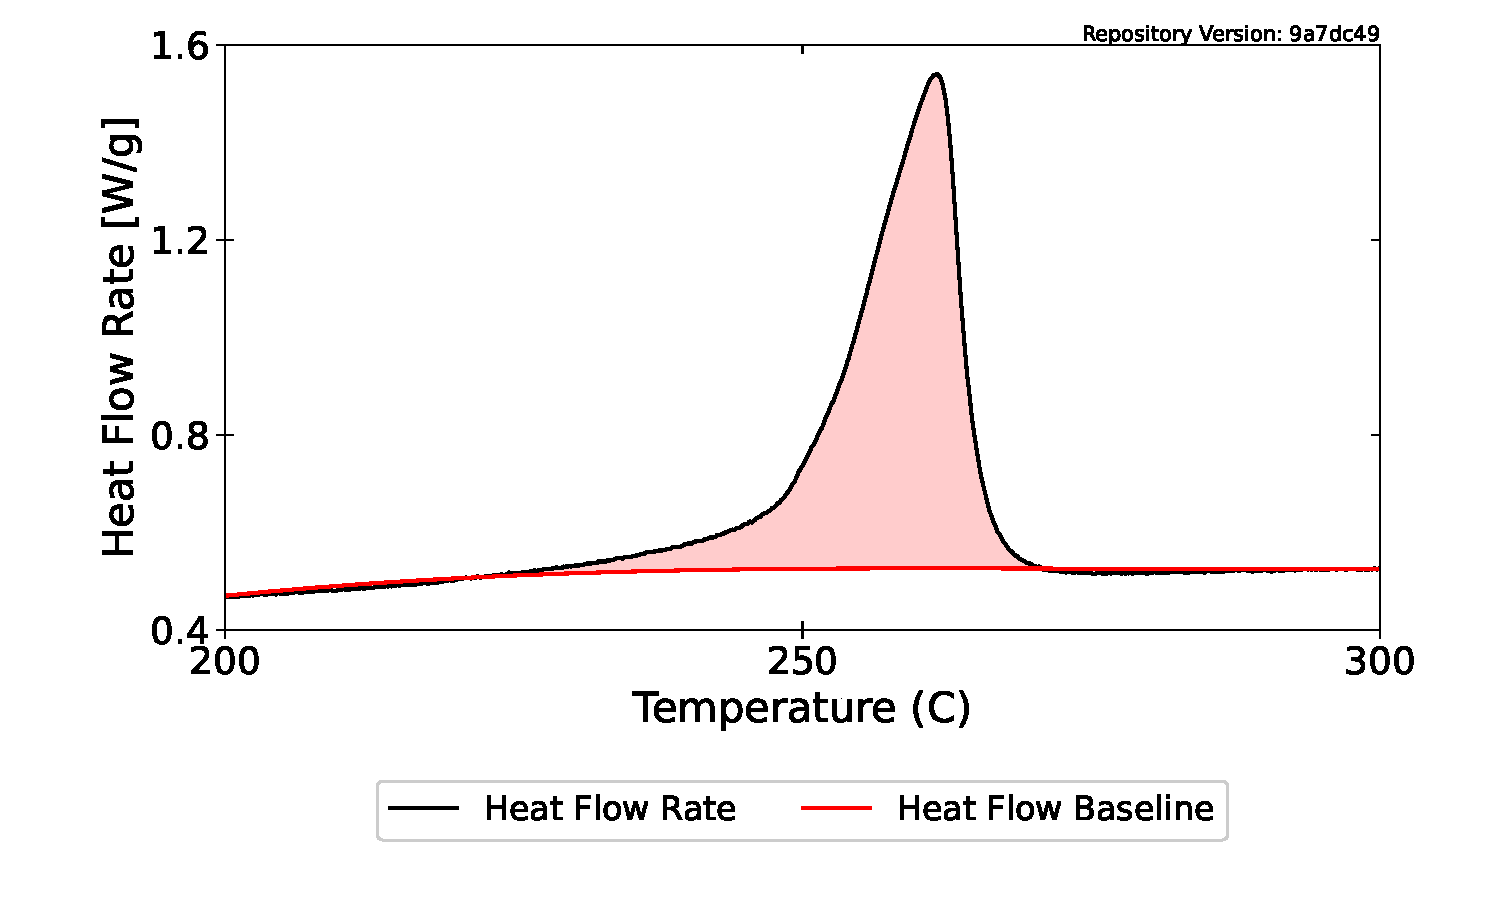
\includegraphics[width=\textwidth]{Figures/Nylon_Melting.pdf}
        \caption{Heat flow rate data for nylon with calculated baseline and melting peak highlighted.}
    \end{subfigure}
    \hfill
    \begin{subfigure}[b]{0.475\textwidth}
        \centering
        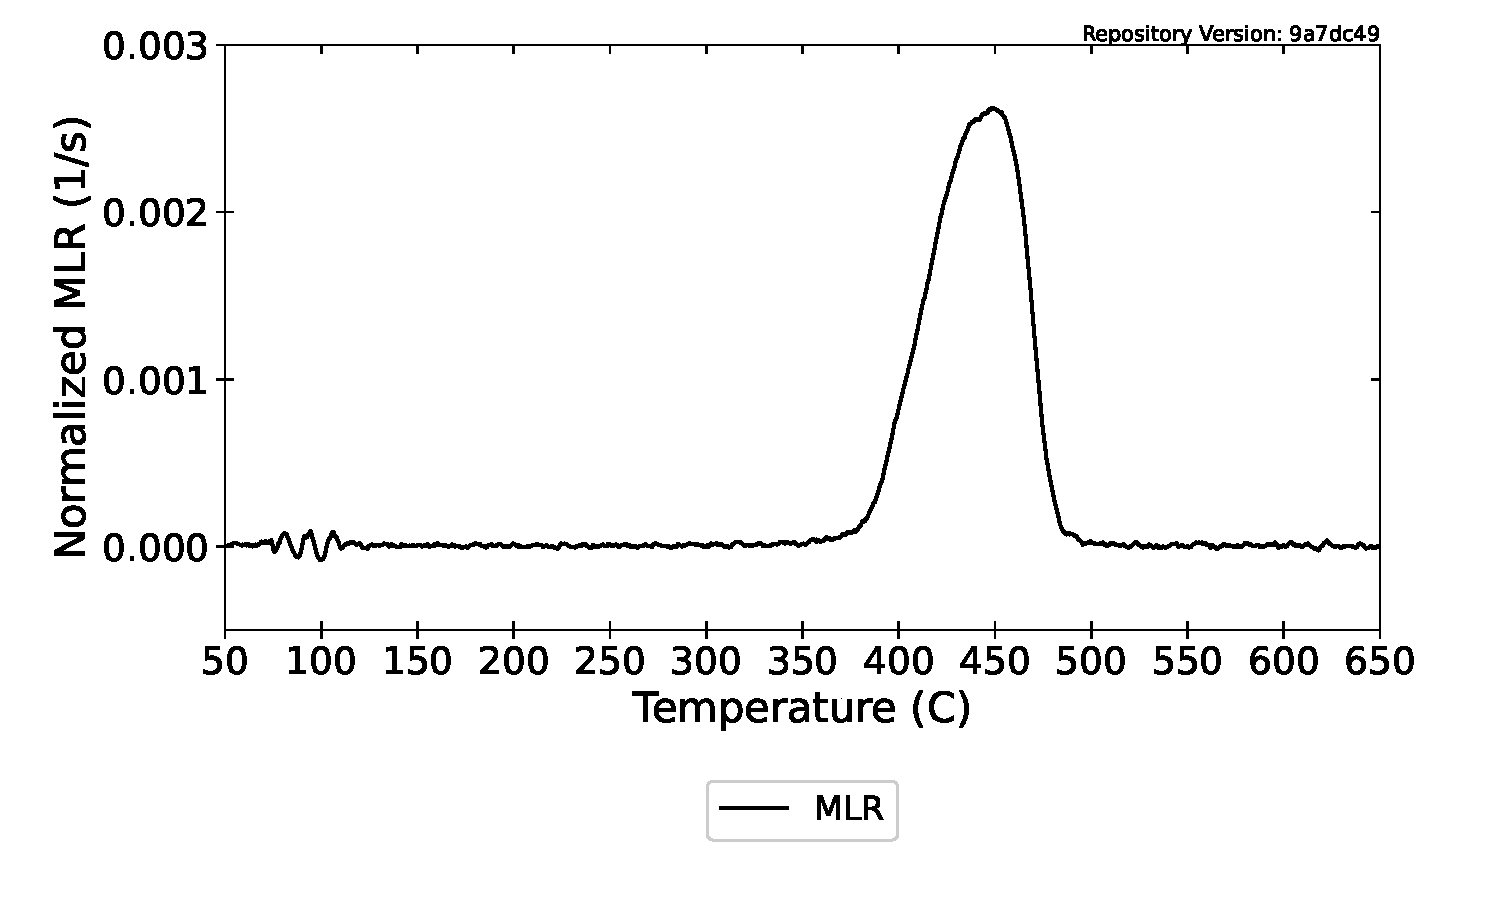
\includegraphics[width=\textwidth]{Figures/Nylon_10K_MLR.pdf}
        \caption{Normalized MLR collected at 10 K/min for nylon.}
    \end{subfigure}
    \caption[Determination of Melting Temperature and Enthalpy of Fusion for Nylon] {Determination of melting temperature and enthalpy of fusion for nylon.} 
    \label{fig:nylon_melting}
\end{figure}

The point at which the data curve deviated from the baseline was determined as the highest temperature below the peak melting temperature at which the two curves intersected and was defined as the temperature at the onset of melting. The point at which the data curve converged back to the baseline was determined in the same way for the temperature above the peak melting temperature at which the curves intersected. The temperature at onset was defined as the lower limit of integration and the the temperature at which the data curve returned to the baseline was defined as the upper limit for the integration. The values measured and calculated for nylon are presented in Table~\ref{tab:melting}.

\begin{table}[!ht]{}
\centering
\caption[Melting Temperature and Enthalpy of Fusion Measured for Nylon]{Melting Temperature and Enthalpy of Fusion Measured for Nylon}
{\begin{tabular}{lc}
\toprule
Measurement       & Nylon   \\
\midrule
Peak Melting Temperature [\degC{ }]       			& 260.8 $\pm$ 0.8		\\ 
Temperature at Onset of Melting [\degC{ }]			& 225 $\pm$ 4			\\
Enthalpy of Melting [J/g]							& 63 $\pm$ 4			\\
\bottomrule
\end{tabular}}
\label{tab:melting}
\end{table}

\section{Heat of Reaction}

The heat of reaction (heat of decomposition) is the amount of energy absorbed by a material during a thermal degradation reaction. The heat of reaction may be determined from STA heat flow rate data according to ASTM E537~\cite{ASTM_E537}. By plotting mass loss rate (MLR) data on the same axes as heat flow rate data, the heat absorbed due to the reaction may be determined. This procedure involves drawing a baseline that connects the heat flow rate curve before the reaction to the heat flow rate curve after the reaction. The heat of reaction is defined as the integral of the difference between the heat flow rate curve and the baseline over the temperature range consistent with the reaction. The heat flow rate data are presented on an initial mass basis, which means the integral must be corrected to represent the total mass lost in the reaction. This is done by multiplying by the initial mass of the sample and dividing by the mass lost in the reaction. 

The trend of the baseline during decomposition is unknown, so often the analysis involves an assumption of the shape of the curve over the temperature range that corresponds to the reaction. Commonly the baseline takes on a linear form or the form of a spline that is tangential at the onset and termination of the reaction. An alternative method of defining the baseline is described by McKinnon et al.~\cite{McKinnon_2013}. With this alternative method, the reaction kinetics and the specific heat capacities of all defined components are used to parameterize a model of the thermal analysis experiment. With a simulation of the mass and composition as a function of temperature, a baseline that represents the sensible enthalpy may be constructed. The baseline calculated with this method for nylon is presented in Figure~\ref{fig:nylon_sensible_enthalpy} along with the heat flow rate data. There is a physical justification for the shape of the baseline when constructed with this procedure. The heats of reaction may be sensitive to the definition of the baseline, but the total heat of gasification is independent of this baseline definition.

\begin{figure}[!ht]
\centering
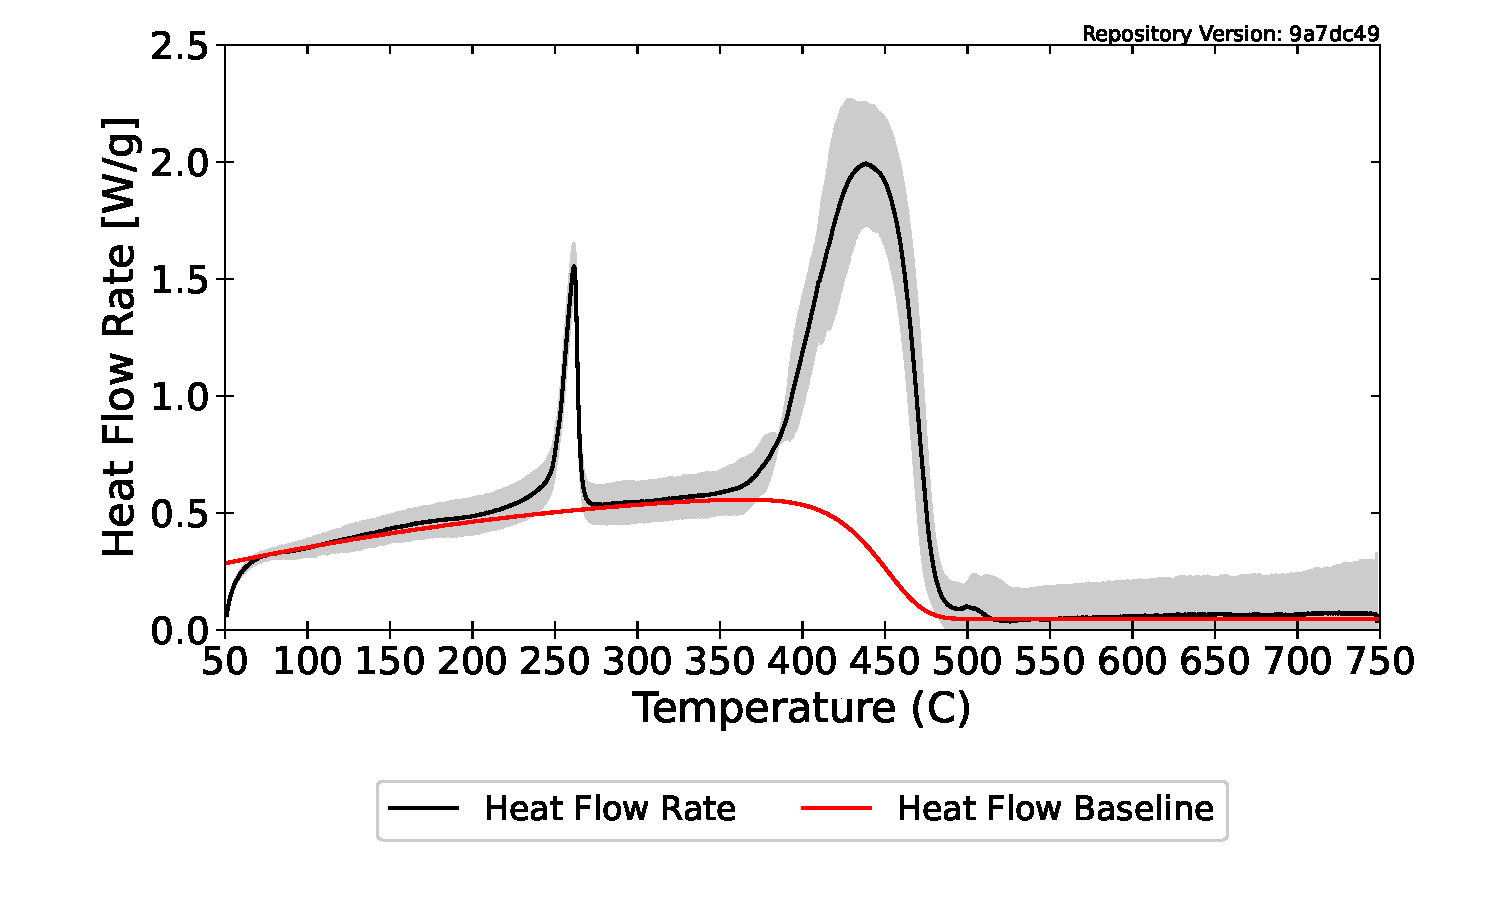
\includegraphics[width=.75\columnwidth]{Figures/Nylon_HR_baseline.pdf}
\caption[Heat flow Rate Data and the Sensible Enthalpy Baseline Calculated for Nylon]{Heat flow rate data and the sensible enthalpy baseline calculated for nylon at 10 K/min.}
\label{fig:nylon_sensible_enthalpy}
\end{figure}

The heat of reaction for the reaction that described decomposition of nylon was determined by integrating between the heat flow rate curve and the sensible enthalpy baseline over the temperature range that corresponded to decomposition. This heat of reaction was calculated as 655 $/pm$ 25 J/g.

\section{Heat of Gasification}

The heat of gasification is defined as the total amount of energy per unit mass required to convert a condensed phase material entirely to the gas or vapor phase. This quantity includes sensible enthalpy (energy required to increase the temperature of the material), heat absorbed during physical transitions, and heat absorbed during decomposition reactions. There are two main approaches to determining the heat of gasification which rely on heat flow rate data collected in thermal analysis experiments and burning rate data collected in bench-scale flammability tests.

Stoliarov and Walters describe a method for determination of the heat of gasification using heat flow rate data collected in experiments conducted in a power compensation DSC~\cite{Stoliarov_2008}. Although the data provided in this database are from experiments conducted with an STA which incorporates a heat flux DSC, the analytical procedure is the same. The heat of gasification is calculated as the integral of the heat flow rate curve (presented in W/g) with respect to time collected in an experiment with a constant heating rate from room temperature to the temperature at which degradation is complete. For the values presented in the database, these integrals were computed over the temperature range of \degC{50} to the temperature at which the MLR decreased to below 5\% of the maximum MLR.

Hopkins and Quintiere describe a method for determination of the heat of gasification from cone calorimeter data~\cite{Hopkins_1996}. According to this method, the peak or quasi-steady burning rate from cone calorimeter tests conducted at a range of incident heat fluxes are plotted with heat flux on the abscissa and mass loss rate on the ordinate. Linear regression is performed and the inverse of the slope of the regression line is considered the effective heat of gasification for non-charring materials. For charring materials, this value must be corrected by dividing by the char mass fraction.

Table~\ref{tab:hog} displays heat of gasification values for nylon and OSB calculated with data collected from the DSC and the cone calorimeter. The method which uses the cone calorimeter data yields a value that is in agreement with the DSC-calculated value, but the values calculated with each method for OSB do not agree. The method that uses cone calorimeter data did not yield a heat of gasification that agreed with the DSC data for OSB. Nylon is a non-charring polymer and is one of the polymers that Hopkins and Quintiere used to validate the calculation method and OSB is a charring lignocellulosic material. Each of these materials was expected to absorb energy and decompose through different mechanisms, so it is not surprising that this analytical technique did not yield consistent results with the DSC data. The method proposed by Hopkins and Quintiere was not used to calculate the heat of gasification for materials other than non-charring thermoplastics. It is evident in the values calculated from DSC data that nylon has a higher heat of gasification, this is a known trend in the comparison between thermoplastics and lignocellulosic materials.

\begin{table}[!ht]{}
\centering
\caption[Heat of Gasification Calculated for Nylon and OSB]{Heat of Gasification Calculated for Nylon and OSB}
{\begin{tabular}{ccc}
\toprule
Material 		& DSC at 10 K/min [J/g]	& Cone Calorimeter [J/g] \\
\midrule
Nylon 			& 1830 $\pm$ 200		& 1648 \\
OSB				& 293 $\pm$ 153			& 8630   \\  
\bottomrule
\end{tabular}}
\label{tab:hog}
\end{table}

\section{HRR}

The HRR of the sample materials was measured with oxygen consumption calorimetry using the cone calorimeter and the MCC. The raw oxygen concentrations measured with each apparatus as well as the analyzed data presented as HRRPUA for the cone calorimeter and specific HRR for the MCC are available in the database. The cone calorimeter measured HRR with respect to time during tests conducted with a set point heat flux incident to the sample. The MCC measured HRR as a function of temperature.

The equation used to calculate the HRR from cone calorimeter data is presented as Equation~\ref{eq:cone_hrr}. $\frac{\Delta{h_c}}{r_o}$ is the heat of combustion of oxygen for the fuel and is typically taken as 13.1 x 10$^3$~kJ/kg by default for materials tested in the cone calorimeter. 1.10 is the ratio of oxygen to air molecular weights. $C$ is the C-factor, which is determined through calibration with the methane flame daily. $\Delta{P}$ is the orifice plate pressure differential and $T_e$ is the absolute temperature of the gas at the orifice plate. $X_{O_2}^0$ is the baseline oxygen volumetric fraction measured immediately prior to the test and $X_{O_2}(t)$ is the instantaneous measured oxygen volume fraction. 1.105 is the volumetric expansion factor that accounts for expansion due to combustion of the air that is depleted of its oxygen. Although this value is dependent on the composition of the fuel and the actual stoichiometry of combustion, 1.105 is a reasonable average that represents the expansion factor due to methane combustion. The 1.5 in the denominator in the last term on the right-hand side of the equation is the stoichiometric expansion factor, which represents the greater number of moles of gas in the products than the number of moles of oxygen consumed in combustion. This factor represents an idealization of the combustion chemistry.

\begin{equation}
\dot{Q}(t) = \left(\frac{\Delta{h_c}}{r_o}\right)(1.10)C\sqrt{\frac{\Delta{P}}{T_e}}\frac{(X_{O_2}^0-X_{O_2}(t))}{1.105-1.5X_{O_2}(t)}  \label{eq:cone_hrr}
\end{equation}

The HRR of the sample pyrolyzate produced in the MCC is measured by oxygen consumption flow calorimetry. The equation used to calculate the HRR is provided as Equation~\ref{eq:mcc_hrr}. The density of gaseous products of combustion ($\rho_{gas}$) is taken as the density of oxygen at \degC{25} and 1~bar. $F$ is the total volumetric flow rate out of the combustion chamber.

\begin{equation}
\dot{Q}(T) = \left(\frac{\Delta{h_c}}{r_o}\right)\left(\frac{\rho_{gas}}{m_0}\right)F(X_{O_2}^0-X_{O_2}(T))  \label{eq:mcc_hrr}
\end{equation}

Figure~\ref{fig:nylon_hrr} displays the HRRPUA measured for nylon at heat fluxes of 25, 50, and 75 kW/m$^2$ as well as the specific HRR measured in MCC experiments. The specific HRR has a maximum value at \degC{462} with a peak magnitude of approximately 270 W/g. Although the total heat released in each cone calorimeter experiment is equal, the HRRPUA curves show a trend where the peak HRRPUA increases and the duration of burning decreases with increasing incident heat flux. This phenomenon is explained with an interpretation of the specific HRR curve such that the temperature of the nylon sample exposed to the cone heater increases in temperature more rapidly at higher incident heat fluxes, which more rapidly increases the specific HRR along its curve, ultimately generating higher HRRPUA values and peaks. 

\begin{figure}[H]
    \centering
    \begin{subfigure}[b]{0.49\textwidth}
        \centering
        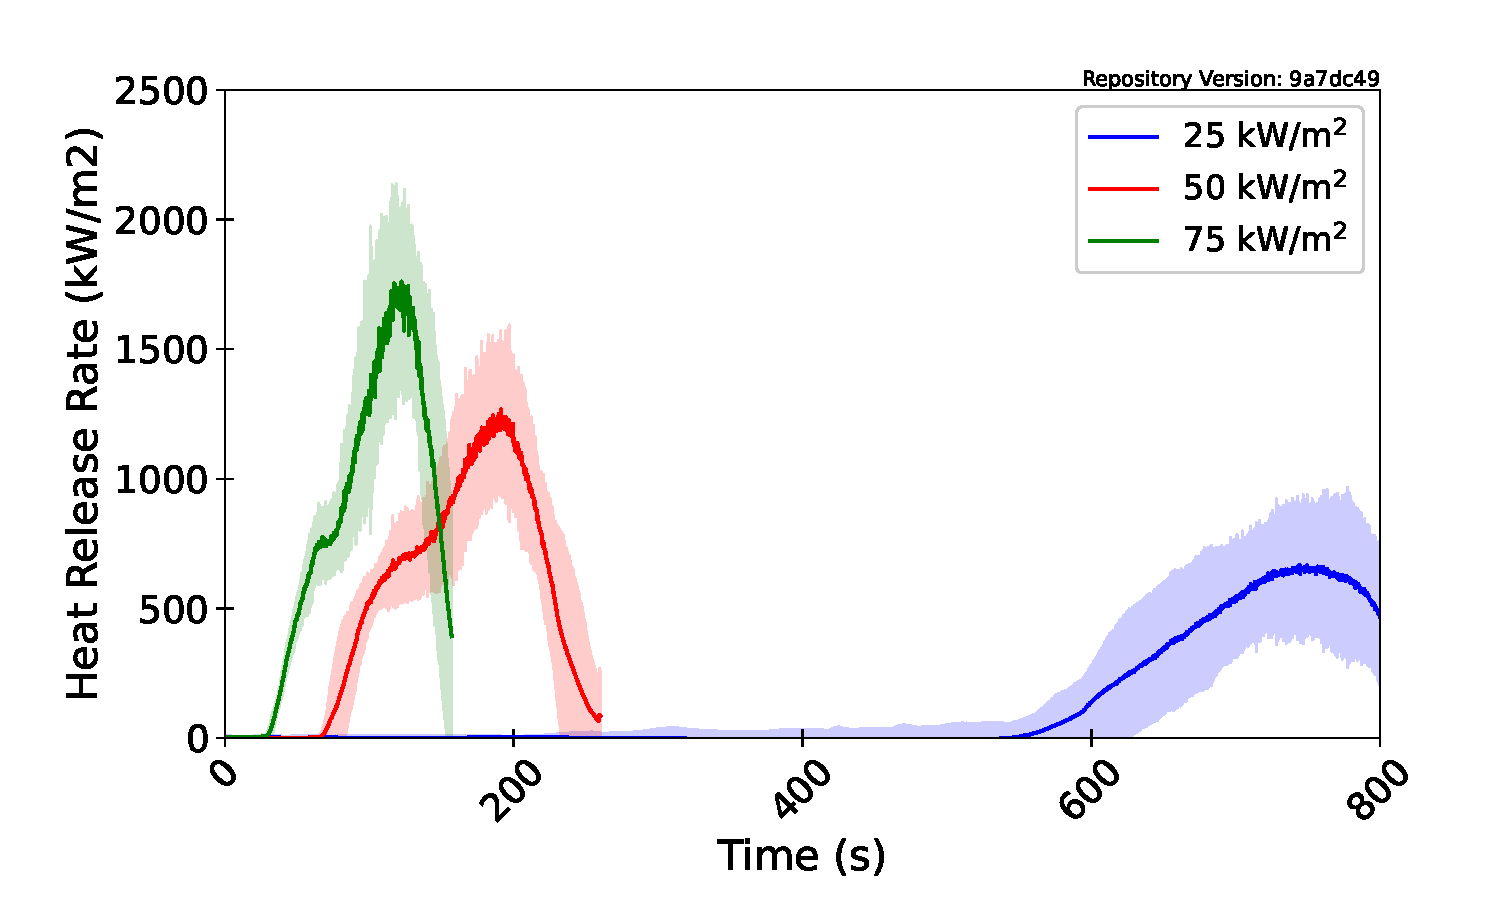
\includegraphics[width=\textwidth]{Figures/Nylon_Cone_HRRPUA_Mean.pdf}
        \caption{HRRPUA measured with the cone calorimeter}
    \end{subfigure}
    \hfill
    \begin{subfigure}[b]{0.49\textwidth}
        \centering
        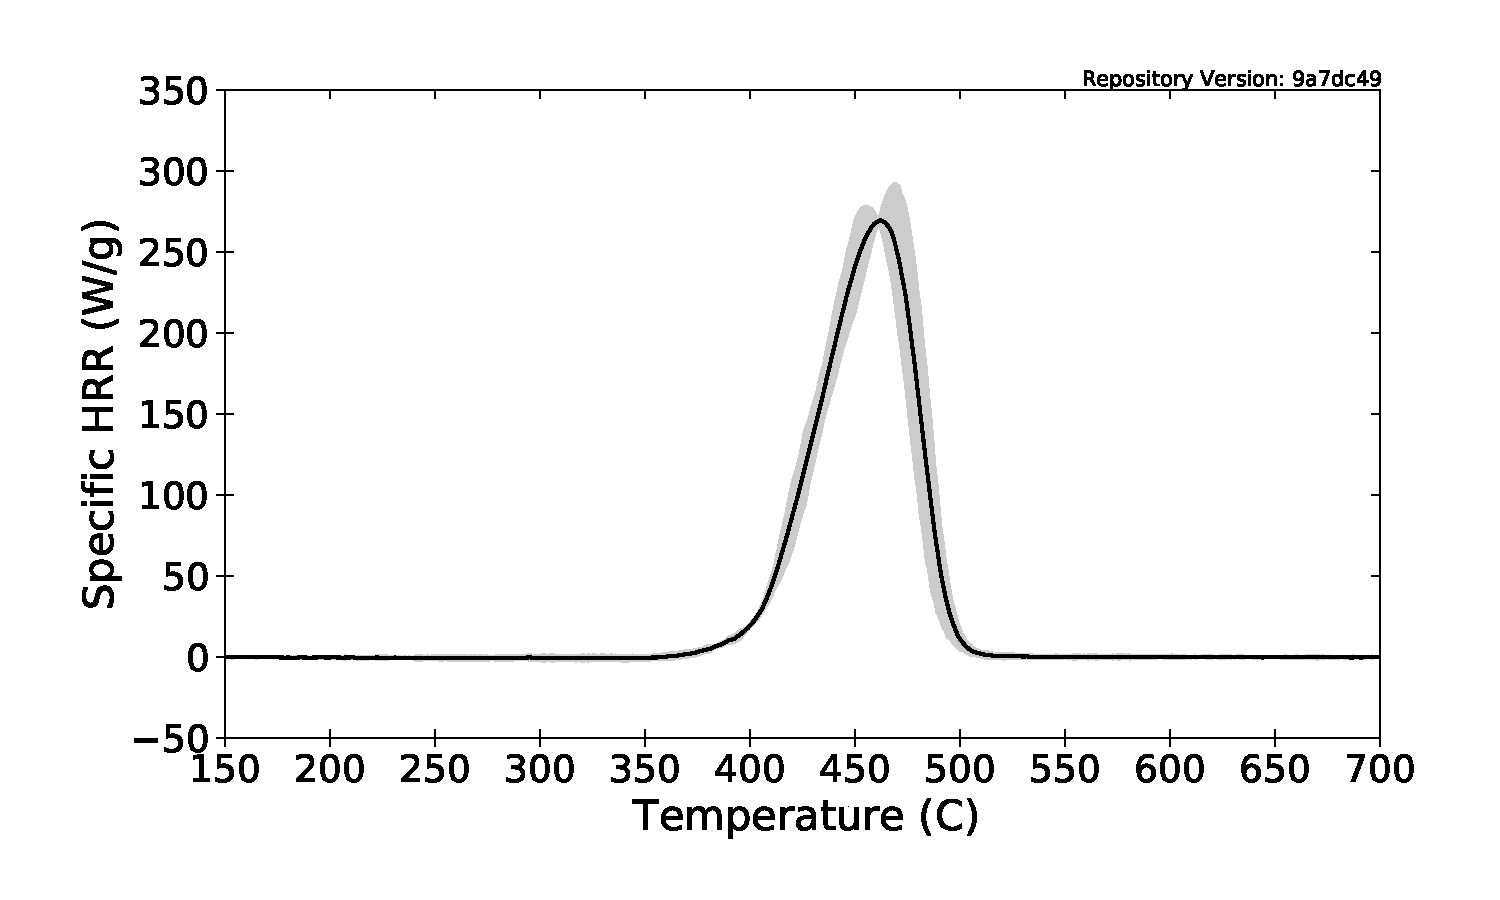
\includegraphics[width=\textwidth]{Figures/Nylon_MCC.pdf}
        \caption{Specific HRR measured with the MCC}
    \end{subfigure}
    \caption[HRR Measured for Nylon] {HRR measured for nylon.} 
    \label{fig:nylon_hrr}
\end{figure}

Figure~\ref{fig:OSB_hrr} displays the HRRPUA measured for (OSB) at heat fluxes of 25, 50, and 75 kW/m$^2$ as well as the specific HRR measured in MCC experiments. The specific HRR has a maximum value at \degC{362} with a peak magnitude of approximately 78 W/g. The same trend in the HRRPUA data from the cone calorimeter that was observed with experiments on nylon is also evident in the data collected on OSB although the peak magnitude of the HRRPUA curves are significantly lower for OSB, which is the same trend observed in the specific HRR data.

\begin{figure}[H]
    \centering
    \begin{subfigure}[b]{0.49\textwidth}
        \centering
        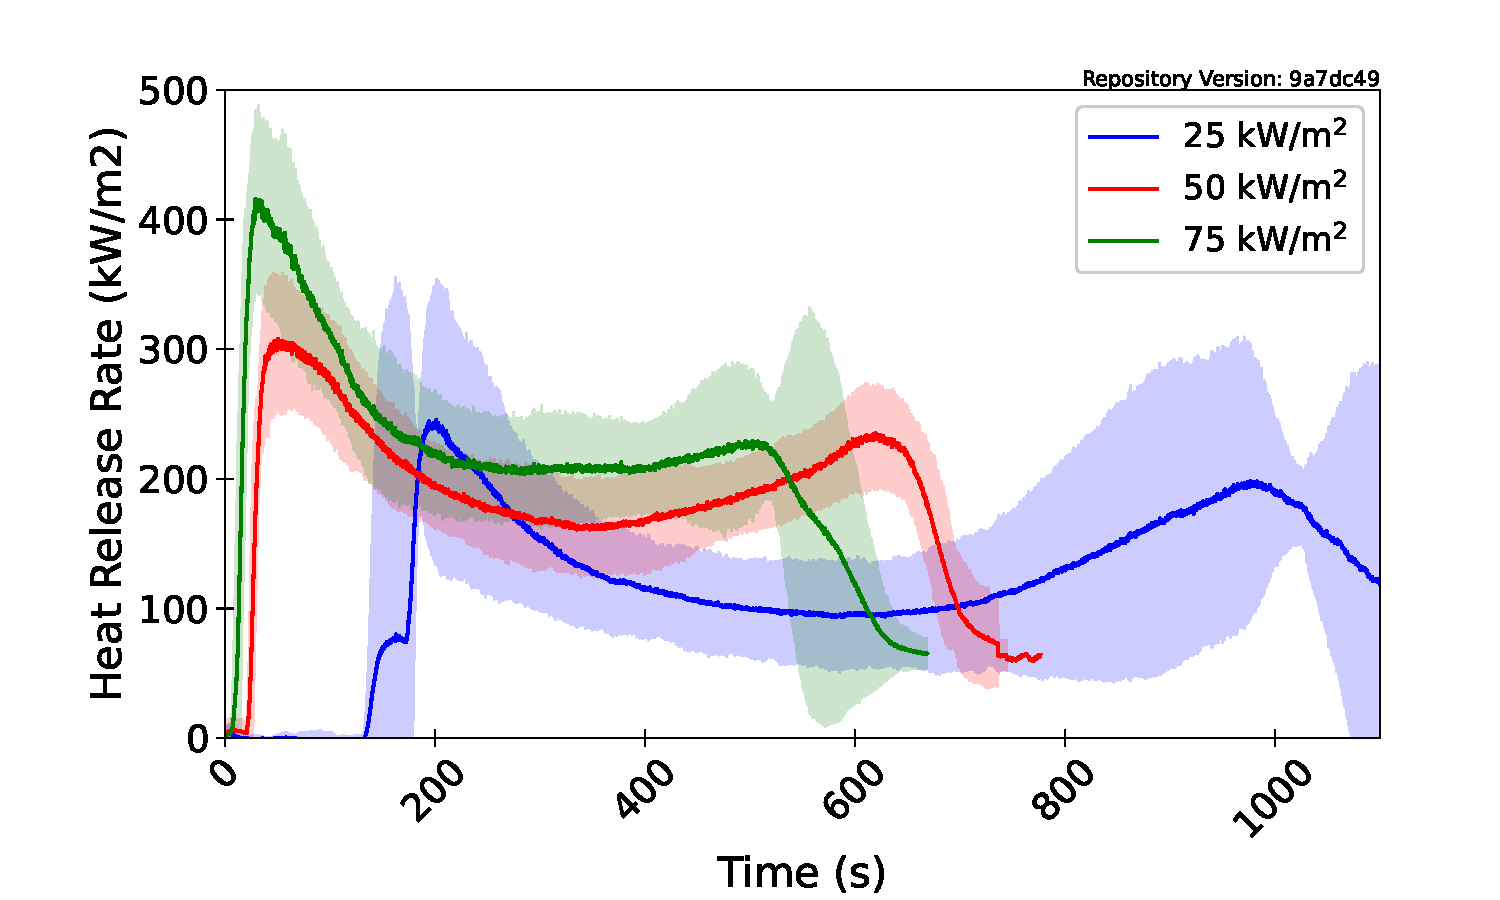
\includegraphics[width=\textwidth]{Figures/OSB_Cone_HRRPUA_Mean.pdf}
        \caption{HRRPUA measured with the cone calorimeter}
    \end{subfigure}
    \hfill
    \begin{subfigure}[b]{0.49\textwidth}
        \centering
        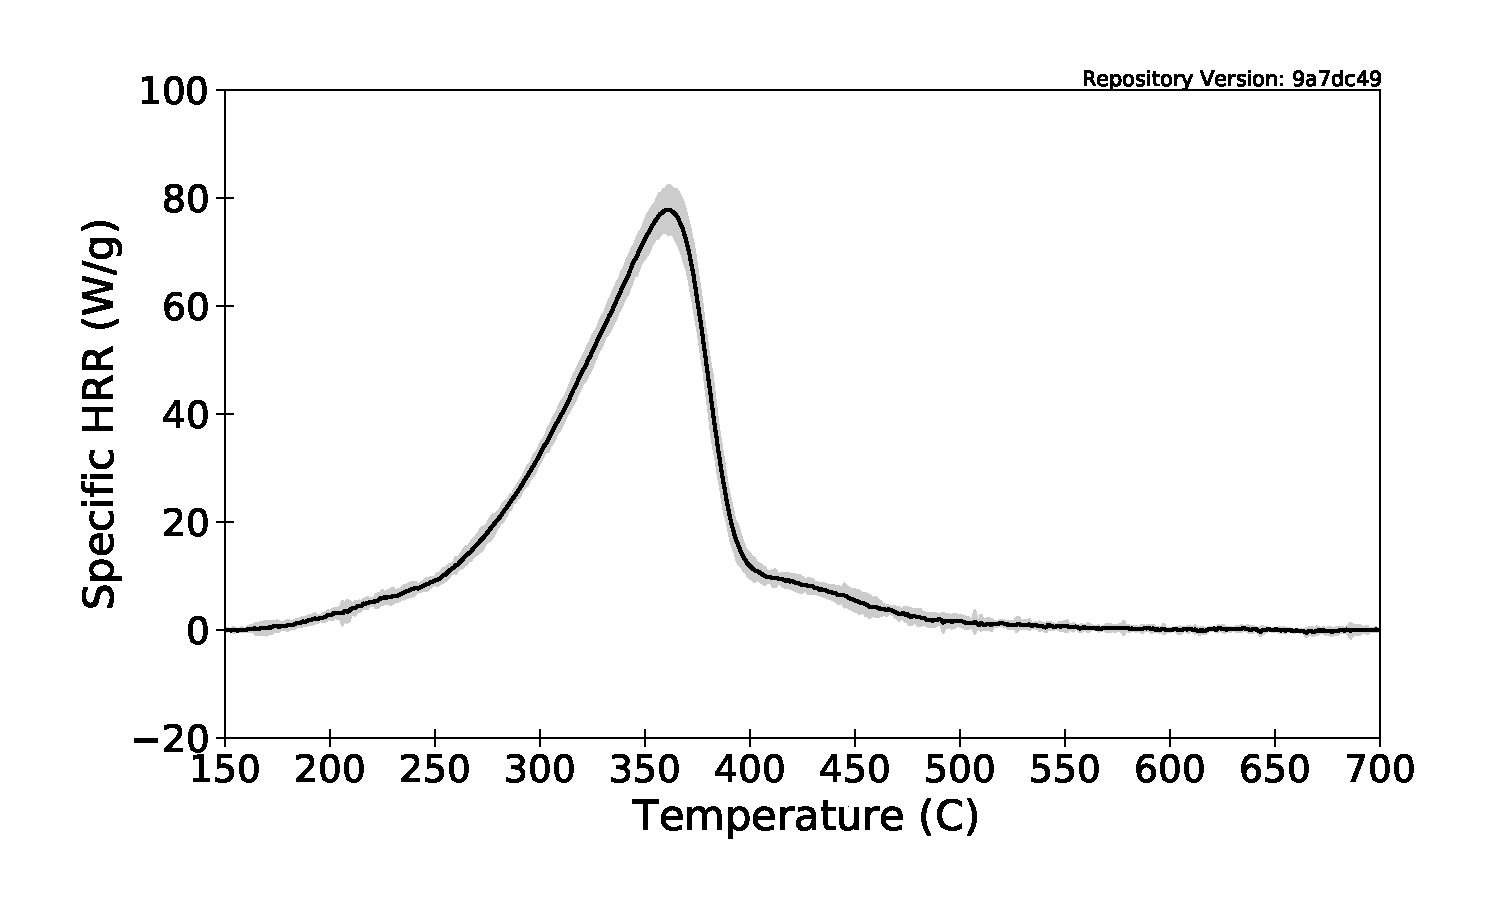
\includegraphics[width=\textwidth]{Figures/OSB_MCC.pdf}
        \caption{Specific HRR measured with the MCC}
    \end{subfigure}
    \caption[HRR Measured for OSB] {HRR measured for OSB.} 
    \label{fig:OSB_hrr}
\end{figure}

\section{Time to Ignition}

The time to ignition is directly observed in cone calorimeter tests as part of the standard test method~\cite{ASTM_E1354}. The times to flashing, sustained ignition, and the time of other pertinent observations about the material being tested at a given set point incident heat flux are saved in the meta data associated with the cone calorimeter tests. The mean time to ignition observed for nylon and OSB in cone calorimeter experiments are provided in Table~\ref{tab:tti}. The time to ignition for OSB is significantly lower than nylon at all tested incident heat fluxes.

\begin{table}[!ht]{}
\centering
\caption[Time to Ignition Observed for OSB and Nylon]{Time to Ignition Observed for OSB and Nylon}
{\begin{tabular}{cccc}
\toprule
Material 	& 25 kW/m$^2$		& 50 kW/m$^2$ 		& 75 kW/m$^2$  \\
\midrule
Nylon 		& 556 $\pm$ 25~s	& 72 $\pm$ 7~s		& 30.3 $\pm$ 0.4~s  \\ 
OSB 		& 161 $\pm$ 23~s 	& 23 $\pm$ 2~s		& 10 $\pm$ 2~s  \\
\bottomrule
\end{tabular}}
\label{tab:tti}
\end{table}

\section{Ignition Temperature}

The ignition temperature is not an intrinsic property of a material. In other words, materials do not spontaneously ignite at a specific universal ignition temperature. The temperature at which materials ignite is a complicated function of the material properties, geometry, orientation, exposure, and environmental conditions. One method that has been proposed to calculate the ignition temperature relies on data collected in the MCC. Several other methods rely on data collected with the cone calorimeter or similar bench-scale flammability experiments. 

A representative ignition temperature is determined from specific HRR data collected with the MCC. Lyon et al.~\cite{Lyon_2018} present a correlation between a critical specific HRR and the temperature for sustained piloted ignition in bench-scale flammability tests. The mean critical specific heat release rate that corresponds to sustained ignition was found to be 25±8 W/g for 20 different polymers. Assuming this correlation applies to other materials that are not synthetic polymers, it may be applied to identify a range of temperatures at which ignition is likely to occur.

\begin{figure}[H]
    \centering
    \begin{subfigure}[b]{0.49\textwidth}
        \centering
        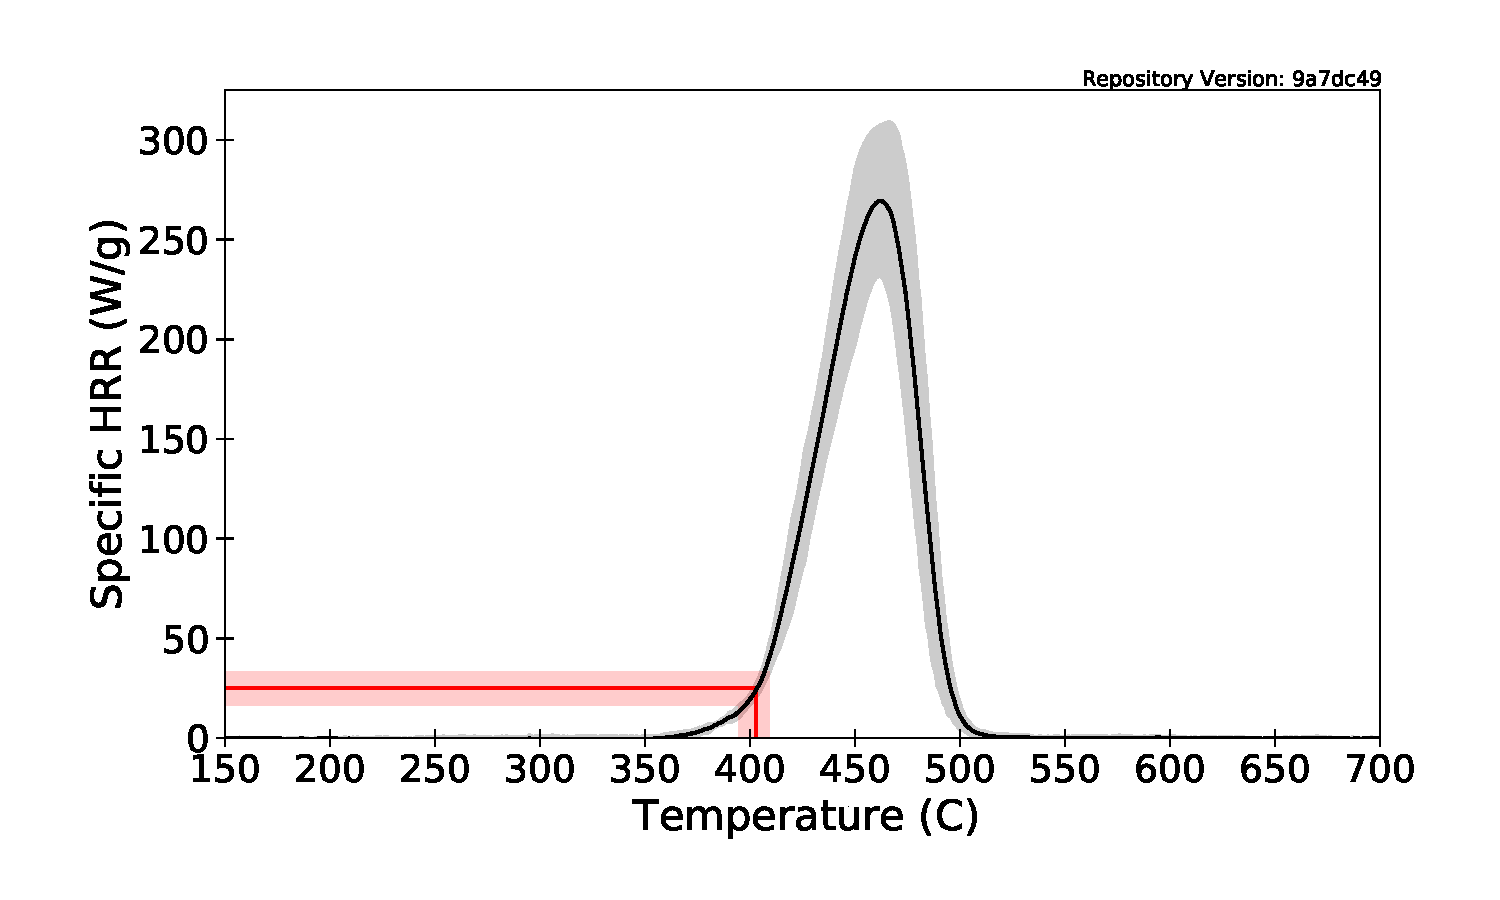
\includegraphics[width=\textwidth]{Figures/Nylon_MCC_Tig.pdf}
        \caption{Application of Lyon's ignition temperature correlation to MCC data for Nylon}
    \end{subfigure}
    \hfill
    \begin{subfigure}[b]{0.49\textwidth}
        \centering
        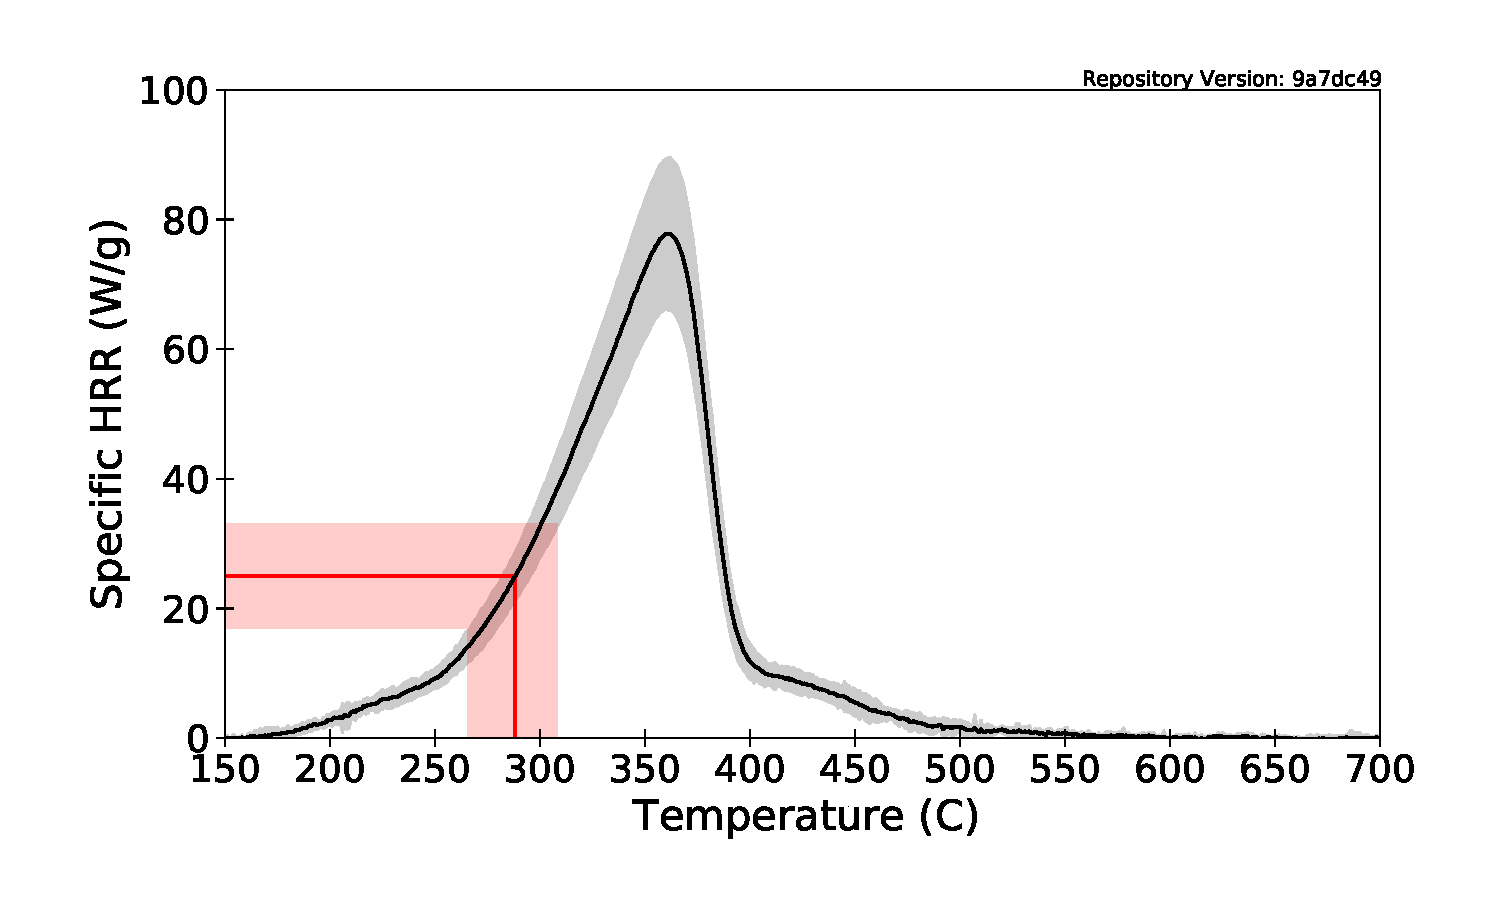
\includegraphics[width=\textwidth]{Figures/OSB_MCC_Tig.pdf}
        \caption{Application of Lyon's ignition temperature correlation to MCC data for OSB}
    \end{subfigure}
    \caption[Application of the Ignition Temperature Correlation for MCC data] {Application of the ignition temperature correlation for MCC data.} 
    \label{fig:mcc_Tig}
\end{figure}

An additional method for calculating the ignition temperature from radiant exposure flammability experiments was developed by Quintiere~\cite{Quintiere}. The equation for the ignition temperature is provided as Equation~\ref{eq:torero_T_ig}, where $T_0$ is the initial temperature of the material, $\dot{q}_e''$ is the heat flux incident to the material, $h_T$ is the total heat transfer coefficient that represents losses from the surface of the material. $t_c$ is defined according to Equation~\ref{eq:torero_t_c}, where $\bar{k}_s$ is the thermal conductivity at the mean surface temperature prior to ignition, $\bar{\rho}_s$ is the density at the mean surface temperature prior to ignition, and $\bar{c}_{p,s}$ is the specific heat capacity at the mean surface temperature prior to ignition.

\begin{equation}
T_{ig} = T_0+\frac{\dot{q}_e''}{h_T}\left[1-e^{\frac{t_{ig}}{t_c}}\text{erfc}\left(\left(\frac{t_{ig}}{t_c}\right)^{\frac{1}{2}}\right)\right]  \label{eq:torero_T_ig}
\end{equation}

\begin{equation}
t_c = \frac{\bar{k}_s\bar{\rho}_s\bar{C}_s}{h_T^2}  \label{eq:torero_t_c}
\end{equation}

There are several other correlations that have been devised to avoid the complementary error function when calculating the ignition temperature and time to ignition using data from the cone calorimeter or similar standard bench-sale flammability tests. DiDomizio et al.~\cite{DiDomizio_2016} provide an excellent discussion of some of the analytical methods that have been used. One such method for estimating the ignition temperature of a material was developed by Tewarson~\cite{Tewarson_2000}. The mathematical relationship between the the time to ignition, the incident heat flux, and the thermo-physical properties of the material is presented as Equation~\ref{eq:tewarson_T_ig}. In the equation, $\dot{q}_e''$ is the heat flux incident to the material, $k$ is the mean thermal conductivity through the material at ignition, $\rho$ is the mean density of the material at ignition, $c_{p,s}$ is the mean specific heat capacity of the material at ignition, $T_{ig}$ is the apparent ignition temperature, $T_\infty$ is the ambient gas temperature, $t_{ig}$ is the observed time to sustained ignition at the given incident heat flux, and $\dot{q}_{cr}''$ is a critical heat flux required for ignition.

\begin{equation}
\dot{q}_e'' = \left(\frac{\pi}{4}\right)^{\frac{1}{2}}\frac{\sqrt{k\rho{c_{p,s}}}(T_{ig}-T_\infty)}{t_{ig}^\frac{1}{2}}+\dot{q}_{cr}''  \label{eq:tewarson_T_ig}
\end{equation}

The critical heat flux in Tewarson's proposed method is defined as the theoretical limiting heat flux at which the time required for sustained ignition approaches infinity. The critical heat flux and the theoretical ignition temperature may be determined by conducting tests with the cone calorimeter or another bench-scale flammability test at several incident heat fluxes and observing the time to ignition with each heat flux. This generally also requires experiments designed specifically to evaluate the critical heat flux where the incident heat flux is incrementally decreased until ignition no longer occurs. The resulting observations are plotted on axes with $t_{ig}^-\frac{1}{2}$ on the ordinate and $\dot{q}_e''$ on the abscissa. If the critical heat flux is not experimentally evaluated, $\dot{q}_{cr}''$ is determined as the intersection of a regression line with the abscissa. $T_{ig}$ may be calculated from the slope of the regression line with knowledge of the thermo-physical properties of the material.

Analytical methods used to calculate the ignition temperature of a material with cone calorimeter data are not currently in the database due to the lack of reliable elevated temperature thermal conductivity.

% \begin{figure}
%     \centering
%     \begin{subfigure}[b]{0.475\textwidth}
%         \centering
%         \includegraphics[width=\textwidth]{04_Charts/hotplate/MDH/emissivity.pdf}
%         \caption{Application of Tewarson's ignition temperature correlation to cone calorimeter data for Nylon}
%     \end{subfigure}
%     \hfill
%     \begin{subfigure}[b]{0.475\textwidth}
%         \centering
%         \includegraphics[width=\textwidth]{04_Charts/hotplate/MDL/emissivity.pdf}
%         \caption{Application of Tewarson's ignition temperature correlation to cone calorimeter data for Luan Paneling}
%     \end{subfigure}
%     \caption[Application of Tewarson's ignition temperature correlation for cone calorimeter data] {\small Application of Tewarson's ignition temperature correlation for cone calorimeter data} 
%     \label{fig:cone_tewarson_Tig}
% \end{figure}

\section{Soot Yield}

The soot yield may be determined from the smoke obscuration measurement in the standard cone calorimeter experiment. Equation~\ref{eq:extinction_coeff} relates the intensity of the laser ($I$) passing through the smoke, relative to a baseline measurement of the intensity of the laser passing through air ($I_0$), to the mass extinction coefficient ($\kappa$), soot density ($\rho_s$), and the path length of the laser ($L$). 

\begin{equation}
\frac{I}{I_0} = \exp{-\kappa\rho_sL}  \label{eq:extinction_coeff}
\end{equation}

To determine the soot yield, the soot density must be determined from the measured decrease in intensity of the laser due to absorption and scattering. The path length of the laser in the cone calorimeter is 0.11~m and Mullholland suggests a value of 8700~m$^2$/kg for the average mass extinction coefficient of smoke~\cite{Mullholland}. The soot density, or mass concentration of soot in air [kg/m$^3$], may be calculated as in Equation~\ref{eq:extinction_coeff_manip}. 

\begin{equation}
\rho_s = \kappa{L}\ln{\frac{I_0}{I}}  \label{eq:extinction_coeff_manip}
\end{equation}

The temperature at the point in the duct where the laser measures the extinction coefficient may be used to calculate the air density. Dividing the mass concentration of soot by the air density yields the mass fraction of soot in the gas mixture. The soot mass fraction may be multiplied by the exhaust duct mass flow rate to yield the total mass flow of soot at a given time in the test. To get the soot yield, the total mass flow of soot in the duct is divided by the mass loss rate of the sample such that the units of yield are [kg of soot produced/kg of sample mass lost]. Equation~\ref{eq:soot_yield} presents this calculation where $\rho_{air}$ is the density of air, $\dot{m}_{exhuast}$ is the exhaust mass flow rate, and $\dot{m}$ is the burning rate of the material.

\begin{equation}
\sigma_s = \frac{\rho_s}{\rho_{air}}\frac{\dot{m}_{exhuast}}{\dot{m}}  \label{eq:soot_yield}
\end{equation}

Table~\ref{tab:soot_yield} displays the soot yields calculated for nylon and OSB from data collected in cone calorimeter experiments at heat fluxes of 25, 50, and 75 kW/m$^2$. The values that are presented in the table and in the database are calculated by integrating the instantaneous soot mass flow rate from the time at which 10\% of the total mass loss has occurred to the time at which 90\% of the total mass loss has occurred and dividing by 80\% of the total mass lost over the test.

\begin{table}[!ht]{}
\centering
\caption[Soot yield Calculated for OSB and Nylon from Cone Calorimeter Experiments]{Soot Yield Calculated for OSB and Nylon from Cone Calorimeter Experiments}
{\begin{tabular}{cccc}
\toprule
Material 		& 25 kW/m$^2$				& 50 kW/m$^2$ 				& 75 kW/m$^2$  \\
\midrule
Nylon 			& 0.032 $\pm$ 0.005 g/g		& 0.020 $\pm$ 0.003 g/g		& 0.014 $\pm$ 0.001 g/g   \\ 
OSB 			& 0.003 $\pm$ 0.001 g/g 	& 0.008 $\pm$ 0.001 g/g		& 0.010 $\pm$ 0.001 g/g    \\
\bottomrule
\end{tabular}}
\label{tab:soot_yield}
\end{table}

\section{Carbon monoxide (CO) Yield}

The carbon monoxide concentration of the effluent collected in the exhaust hood of the cone calorimeter is typically measured during an experiment. This concentration is reported in parts per million (ppm) or as a volumetric concentration. To convert from volumetric fraction to mass fraction, the volumetric fraction must be multiplied by the ratio of the density of carbon monoxide to the density of air flowing through the duct. This resulting mass fraction is multiplied by the exhaust duct mass flow rate to get the instantaneous mass flow rate of CO. The instantaneous CO yield [kg of CO produced/kg of sample mass lost] may be determined by dividing the mass flow rate of CO in the duct by the mass loss rate of the sample. Equation~\ref{eq:co_yield} presents this calculation where $X_{CO}$ is the instantaneous volumetric fraction of CO measured in the experiment, $\rho_{CO}$ is the density of CO, $\rho_{air}$ is the density of air, $\dot{m}_{exhuast}$ is the exhaust mass flow rate, and $\dot{m}$ is the burning rate of the material.

\begin{equation}
\sigma_{CO} = X_{CO}\frac{\rho_{CO}}{\rho_{air}}\frac{\dot{m}_{exhuast}}{\dot{m}}  \label{eq:co_yield}
\end{equation}

Table~\ref{tab:co_yield} displays the CO yields calculated for nylon and OSB from data collected in cone calorimeter experiments at heat fluxes of 25, 50, and 75 kW/m$^2$. The values that are presented in the database are calculated by integrating the instantaneous soot mass flow rate from the time at which 10\% of the total mass loss has occurred to the time at which 90\% of the total mass loss has occurred and dividing by 80\% of the total mass lost over the test.

\begin{table}[!ht]{}
\centering
\caption[CO yield Calculated for OSB and Nylon from Cone Calorimeter Experiments]{CO yield Calculated for OSB and Nylon from Cone Calorimeter Experiments}
{\begin{tabular}{cccc}
\toprule
Material 			& 25 kW/m$^2$				& 50 kW/m$^2$ 				& 75 kW/m$^2$  \\
\midrule
Nylon 				& 0.007 $\pm$ 0.007 g/g		& 0.008 $\pm$ 0.008 g/g		& 0.013 $\pm$ 0.002 g/g   \\ 
OSB 				& 0.008 $\pm$ 0.006 g/g 	& 0.005 $\pm$ 0.002 g/g		& 0.007 $\pm$ 0.001 g/g    \\
\bottomrule
\end{tabular}}
\label{tab:co_yield}
\end{table}

\section{Heat of Combustion}

The heat of combustion is defined as the amount of energy released when the pyrolyzate gases produced during pyrolysis of a material undergo combustion. The heat of combustion is typically presented on a per unit mass of the condensed phase material basis. An effective heat of combustion may be calculated from cone calorimeter data and an effective heat of complete combustion may be determined from analysis of MCC HRR data. Because the cone calorimeter experiments are conducted in an open atmosphere with a potentially turbulent flame and the temperature and oxygen concentration in the MCC combustion chamber are well controlled, the process and efficiency of combustion for these two scenarios are significantly different. Typically, the effective heat of combustion measured in the cone calorimeter incorporates some incomplete combustion that produces soot and carbon monoxide and the resultant value is lower than the theoretical heat of combustion. In the MCC, combustion is forced through completion, and so the effective heat of combustion is typically closer to the theoretical value. 

The instantaneous effective heat of combustion may be calculated from cone calorimeter data by dividing the instantaneous HRR by the instantaneous mass loss rate. A representative value may also be determined from the duration of the cone calorimeter test by dividing the total heat release (integral of HRR) by the total mass lost.

Because the mass of the sample specimen is not monitored during the test in the MCC, an effective heat of complete combustion may be calculated after a test in completed. The total heat released over the duration of the test is divided by the total mass lost (difference of initial mass and residual mass) to get the heat of complete combustion.

Table~\ref{tab:hoc} displays the heats of combustion for nylon and OSB calculated with MCC data and cone calorimeter data. The values calculated with each method are in agreement, with the effective heat of combustion measured in the cone calorimeter slightly higher than the heat of complete combustion measured with the MCC for both materials. The heat of combustion of nylon is at least twice that of OSB. The trend of higher heats of combustion for thermoplastics than lignocellulosic materials is well known and these results are consistent with that trend. 

\begin{table}[!ht]{}
\centering
\caption[Heat of Combustion Calculated for Nylon and OSB]{Heat of Combustion Calculated for Nylon and OSB}
{\begin{tabular}{ccc}
\toprule
Material 		& MCC [kJ/g]	& Cone Calorimeter [kJ/g] \\
\midrule
Nylon  			& 30 $\pm$ 1	& 35 $\pm$ 2 \\
OSB 			& 14 $\pm$ 1	& 15 $\pm$ 1  \\
\bottomrule
\end{tabular}}
\label{tab:hoc}
\end{table}

\section{Thermal Conductivity}

Thermal conductivity was directly measured and no analysis was required to get a final value for thermal conductivity.

\begin{table}[!ht]{}
\centering
\caption[Thermal Conductivity of Nylon and OSB]{Thermal Conductivity of Nylon and OSB Measured with the HFM}
{\begin{tabular}{cccc}
\toprule
Material 						& \degC{15} [W/m-K]		& \degC{45} [W/m-K] 	& \degC{65} [W/m-K] \\
\midrule
Nylon (Unconditioned) 			& 0.142 $\pm$ 0.016		& 0.154 $\pm$ 0.016		& N/T 				 \\
Masonite (Unconditioned)		& 0.106 $\pm$ 0.006		& N/T					& 0.124 $\pm$ 0.004  \\
Masonite (Dried) 				& 0.096 $\pm$ 0.008		& N/T					& 0.110 $\pm$ 0.008  \\  
\bottomrule
\end{tabular}}
\label{tab:conductivity}
\end{table}

\section{Emissivity}

Total broadband emissivity was calculated from spectral reflectance data collected with the integrating sphere. The emissivity was taken as equal to the absorptance through Kirchoff's Law, and the majority of the materials were assumed to act as opaque bodies, which allows definition of the absorptance equal to one minus the reflectance of the material. The materials that were transparent to visible light were also assumed to be non-opaque to infrared radiation. For these materials, the absorptance was defined as one minus the transmittance minus the reflectance of the material. For the materials that could not be defined as opaque to infrared radiation, the absorption coefficient was determined according to the analytical procedure presented in the following section. The emissivity was calculated according to Equation~\ref{eq:emissivity}, where $\epsilon_{\lambda,s}$ denotes the spectral emittance of the sample, $r_{\lambda,s}$ is the spectral reflectance of the sample, and $r_{\lambda,ref}$ is the spectral reflectance of the light trap.

\begin{equation}
\epsilon_{\lambda, s} = 1 - \frac{r_{\lambda,s}-r_{\lambda,ref}}{1-r_{\lambda,ref}} - \tau_{\lambda, s} \label{eq:emissivity}
\end{equation}

To calculate the total emissivity for the material, the resulting spectral emittance must be integrated with respect to wavelength or wavenumber. An appropriate weighting function is required to scale the spectral emittance so that all wavelengths are not equally weighted. This weighting function takes the form of Planck's law (Equation~\ref{eq:planck}), which describes the radiant power from a source per wavelength over a given solid angle, $I_s$, in W/sr-m$^3$ as a function of temperature, $T$, in K and wavelength, $\lambda$, in m. In the equation, $h$ is the Planck constant [6.62e-34 J-s], $c$ is the velocity of light in air [2.997e8 m/s], $k_B$ is the Boltzmann constant [1.381e-23 J/K].

\begin{equation}
I_s(\lambda) = \frac{2\pi{h}c^2}{\lambda^5}\frac{1}{\exp\left(\frac{hc}{\lambda{k_B}T}\right)-1} \label{eq:planck}
\end{equation}

The radiant power of the theoretical source was evaluated at several temperatures in a range that may be representative of an enclosure fire (600~K to 2000~K). The curve produced from Planck's Law calculated with the given source temperature (Figure~\ref{fig:reference_spectra}) was used to scale the calculated spectral emissivity and the integral of the scaled emissivity was taken as the total band-averaged emissivity at the source temperature. The plot shows that the peak of the spectral curves shifts to higher wavelengths as the source temperature decreases. This has particular implications for spectral emissivity measured below 2500~nm, which is weighted more heavily for high source temperatures. 

\begin{figure}[!ht]
\centering
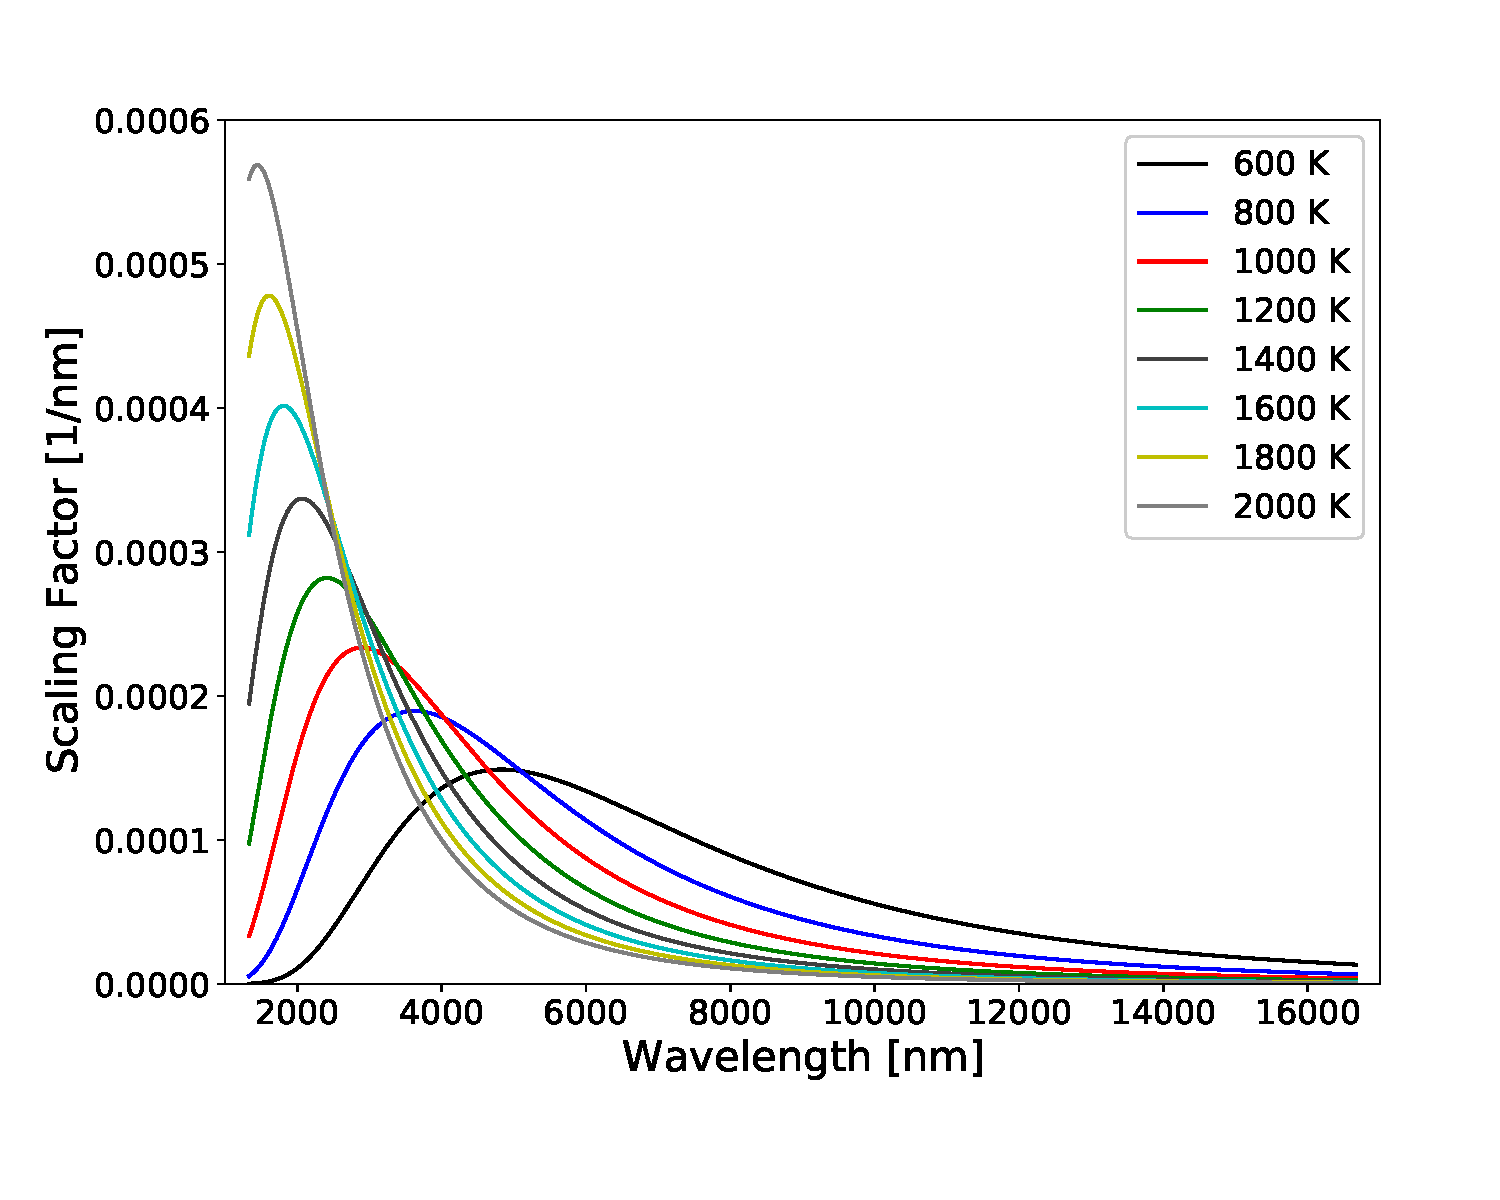
\includegraphics[width=.75\columnwidth]{Figures/Nylon_Spectral_Curves.pdf}
\caption[Reference Spectral Curves at a Range of Source Temperatures]{Reference spectral curves at a range of source temperatures.}
\label{fig:reference_spectra}
\end{figure}

Because the nylon that was tested was translucent to visible light, it was hypothesized that infrared radiation was transmitted through the material along with visible light. The spectral transmittance was measured along with the reflectance to calculate the spectral emittance. The measured spectral emittance is plotted in Figure~\ref{fig:nylon_emittance}. The emittance for nylon is relatively wavelength-independent, which means there is not likely to be a strong source temperature dependence of the calculated broadband emissivity. 

\begin{figure}[!ht]
\centering
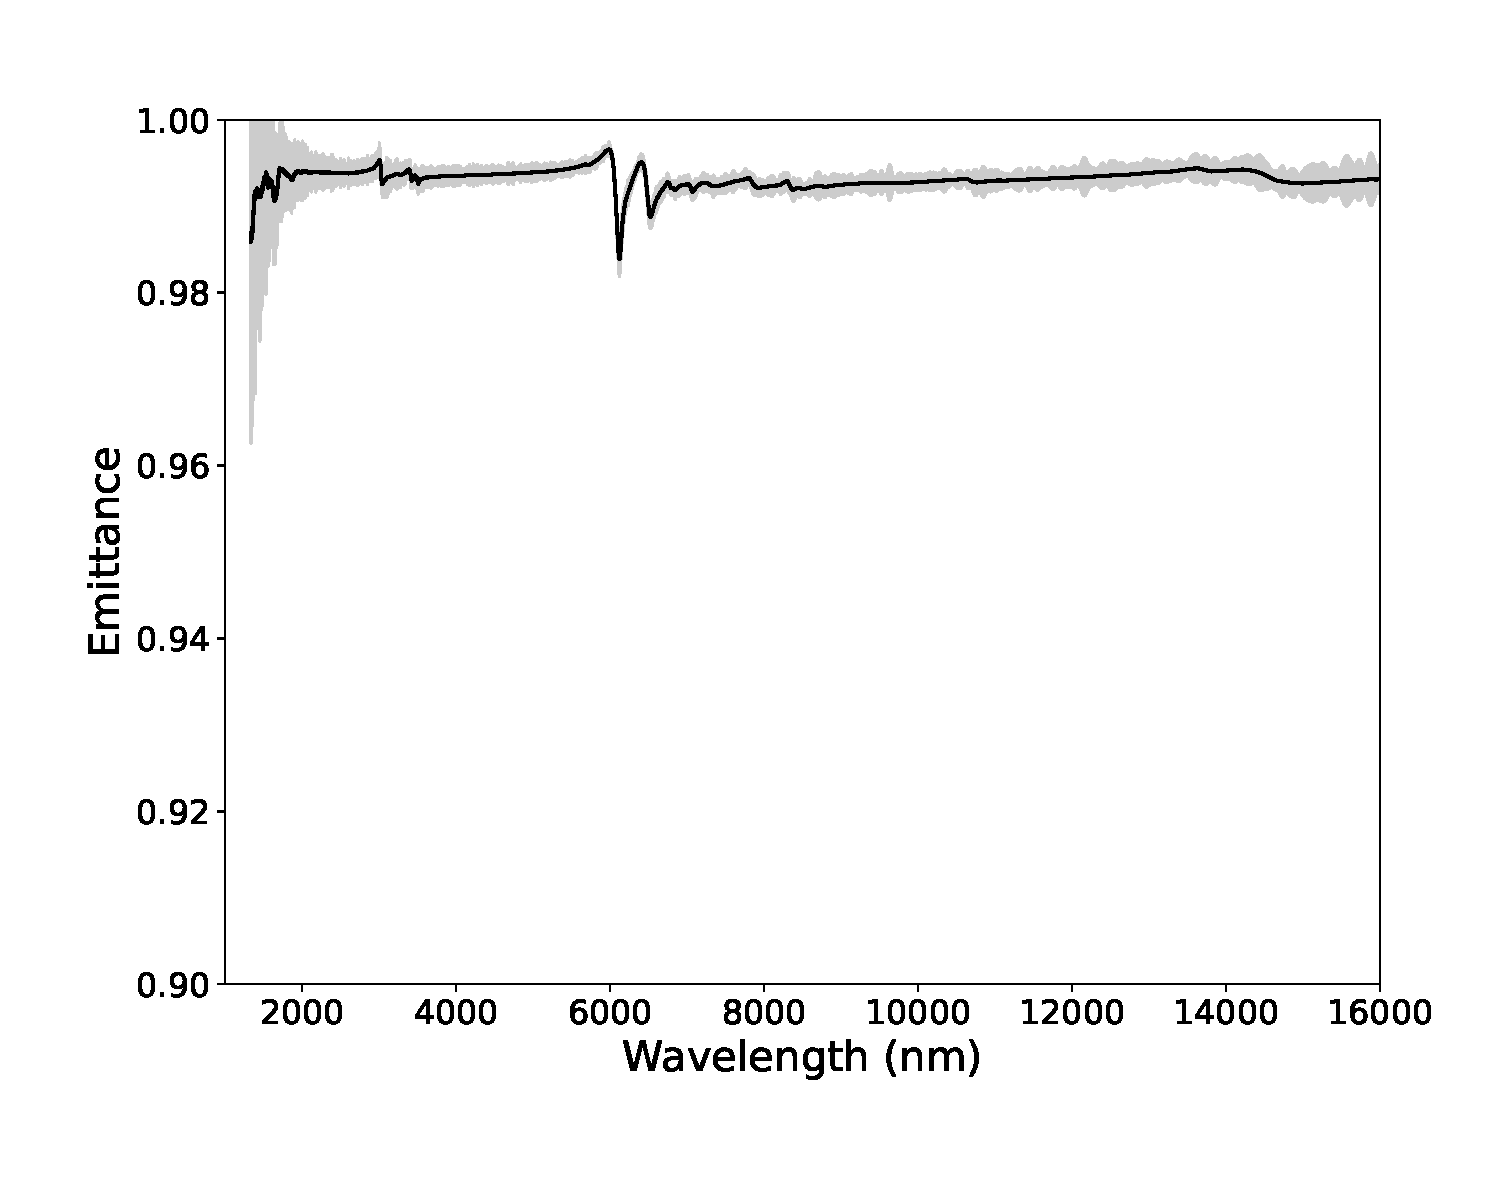
\includegraphics[width=.75\columnwidth]{Figures/Nylon_Measured.pdf}
\caption[Measured Spectral Emittance for Nylon]{Measured spectral emittance for nylon.}
\label{fig:nylon_emittance}
\end{figure}

The broadband emissivity was determined by multiplying the spectral emittance by the weighting function curves specific to each source temperature and integrating the product with respect to the wavelength. This result was normalized by the integral of the weighting function curve to ensure the resulting integral was unitless. Table~\ref{tab:nylon_emissivity} presents the source temperature-dependent broadband emissivity for nylon and masonite. Masonite was assumed to be opaque to infrared radiation, so transmittance was not measured.

\begin{table}[!ht]{}
\centering
\caption[Source Temperature-Dependent Broadband Emissivity]{Source Temperature-Dependent Broadband Emissivity Calculated for Nylon and Masonite}
{\begin{tabular}{ccc}
\toprule
Source Temperature [K]	& Nylon						& Masonite					\\
\midrule
600						& 0.993 $\pm$ 0.002			& 0.970 $\pm$ 0.002			\\ 
800						& 0.989 $\pm$ 0.002			& 0.960 $\pm$ 0.002			\\
100						& 0.978 $\pm$ 0.002			& 0.945 $\pm$ 0.004			\\
1200					& 0.961 $\pm$ 0.002			& 0.928 $\pm$ 0.004			\\ 
1400					& 0.942 $\pm$ 0.002			& 0.911 $\pm$ 0.004			\\
1600					& 0.923 $\pm$ 0.002			& 0.896 $\pm$ 0.006			\\
1800					& 0.906 $\pm$ 0.002			& 0.883 $\pm$ 0.006			\\ 
2000					& 0.891 $\pm$ 0.002			& 0.873 $\pm$ 0.006			\\
\bottomrule
\end{tabular}}
\label{tab:nylon_emissivity}
\end{table}

\section{Absorption Coefficient}

For materials that are not opaque to infrared radiation, it is important to quantify the fraction of incident radiation that is transmitted through the material or absorbed in depth. Linteris et al. provide a discussion of attenuation of radiation within a medium~\cite{Linteris:2011}. The absorption coefficient is a metric that quantifies the amount of infrared radiation absorbed by a material and may be considered the inverse of the mean penetration depth [1/m] or the same quantity normalized by the density of the material [m$^2$/kg]. A large absorption coefficient indicates all the radiation is absorbed at the exposed surface of the material or close to the surface of the material. The form of Bouger's law that may be applied to describe the transmittance of a material is provided as Equation~\ref{eq:transmittance}, where $\tau_\lambda(S)$ is the spectral transmittance at a given path length, $I_\lambda$ is the spectral intensity measured by the detector attached to the integrating sphere, $S$ is the path length through the sample [m], and $\kappa_\lambda$ is the spectral absorption coefficient [1/m].

\begin{equation}
\tau_\lambda(S) = \frac{I_\lambda(S)}{I_\lambda(0)} = \exp\left(-\kappa_\lambda{S}\right) \label{eq:transmittance}
\end{equation}

The equation was manipulated into the linear form of Equation~\ref{eq:transmittance_lin} to simplify determination of the absorption coefficient.

\begin{equation}
-\ln\left(\tau\right) = \kappa{S} \label{eq:transmittance_lin}
\end{equation}

Transmittance was measured for samples of several thicknesses relative to the light trap and complete transmission (no sample in the integrating sphere). The mean total transmittance was calculated by integrating the spectral transmittance over the range of wavelengths at which the measurement was made scaled by the blackbody spectrum from a range of source temperatures. The thickness of the sample was plotted against the negative of the natural logarithm of the average total transmittance and linear regression was performed. The slope of the regression line was taken as the absorption coefficient for the material when exposed to radiation at the specific source temperature. Figure~\ref{fig:nylon_absorption_coefficient} displays the graphical procedure used to calculate the absorption coefficient of nylon for a source temperature of 1600~K. Table~\ref{tab:nylon_absorption_coefficient} displays the source temperature-dependent absorption coefficient calculated for for nylon exposed to a source at each temperature.

\begin{figure}[!ht]
\centering
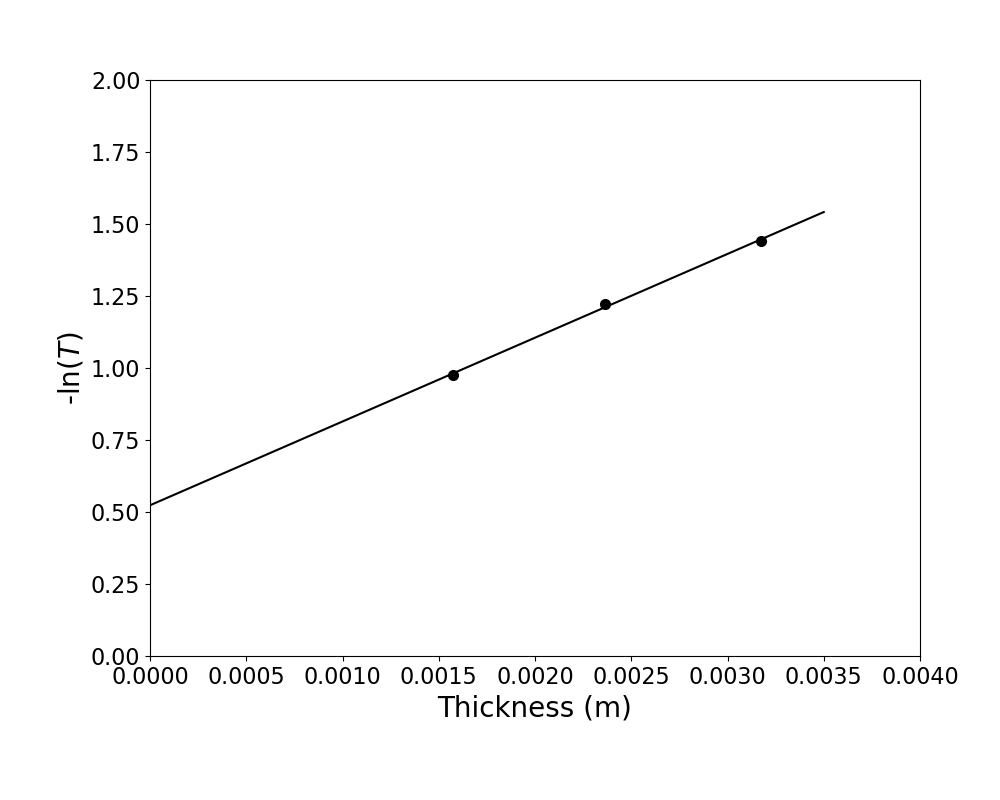
\includegraphics[width=.75\columnwidth]{Figures/Nylon_Absorption_coefficient.png}
\caption[Graphical Procedure to Determine Absorption Coefficient for Nylon]{Graphical procedure to determine absorption coefficient for nylon.}
\label{fig:nylon_absorption_coefficient}
\end{figure}

\begin{table}[!ht]{}
\centering
\caption[Source Temperature-Dependent Absorption Coefficient]{Source Temperature-Dependent Absorption Coefficient}
{\begin{tabular}{cc}
\toprule
Source Temperature [K]			& Nylon	\\
\midrule
600						& 2900 $\pm$ 300\\ 
800						& 720 $\pm$ 270	\\
1000					& 540 $\pm$ 100	\\
1200					& 460 $\pm$ 60	\\ 
1400					& 420 $\pm$ 50 \\
1600					& 400 $\pm$ 40	\\
1800					& 376 $\pm$ 36	\\ 
2000					& 363 $\pm$ 34	\\
\bottomrule
\end{tabular}}
\label{tab:nylon_absorption_coefficient}
\end{table}

\bibliography{../Bibliography/MaP_Database_Bibliography}

\end{document}